\chapter{Simulazioni}
\label{cap:simulazioni}
In questo capitolo vengono presentate in dettaglio le simulazioni effettuate in SIL e MIL. Inoltre è presente una sezione in cui verrà riportata parzialmente la soluzione per le simulazioni in PIL. Nella sezione di MIL verrà descritto il modello dei sensori e dello stimatore usato nella precedente tesi, \cite{DesTestCarm}, per il confronto. Diverse osservazioni e confronti verranno fatti tra le simulazioni. La parte finale descriverà la conclusione del lavoro e eventuali sviluppi futuri.

Nelle simulazioni verranno utilizzati i seguenti percorsi:
\begin{itemize}
		\item \textbf{STEP: } Questa sequenza di waypoint definisce una fase di decollo stazionando a 3 m dal suolo, Tabella (\ref{tab:STEP})
		\item \textbf{SQUARE: } Sequenza di decollo seguita da un percorso a 2.5 m di altezza di forma quadrata con lato di 3 m e atterraggio nell'ultima posizione, Tabella (\ref{tab:SQUARE})
		\item \textbf{BUTTERFLY: } Sequenza di decollo seguita da un percorso a croce su un area di 3 m per lato, Tabella (\ref{tab:BUTTERFLY})
		\item \textbf{SNAKE: } Sequenza di decollo fino a 2.5 m, seguita da un percorso di forma varia descritta nella Tabella (\ref{tab:SNAKE})
\end{itemize}

\section{Simulazione SIL}

\begin{figure}
	\centering
	\includegraphics[width=1\textwidth]{DescrizioneAutopilota/Figure/SIMSIL}
	\caption{Descrizione del procedimento per effettuare la simulazione SIL}
	\label{fig:SIMSIL}
\end{figure}

Per effettuare la simulazione è necessaria la generazione del codice, processo che avviene in modo automatico utilizzando Simulink. Dopo aver selezionato nell'apposito file di inizializzazione la sequenza di waypoint necessari per la generazione della traiettoria, si lancia una prima fase di simulazione standard, come riportato nella guida, \cite{px4Guide}. Si termina il software lanciato dal tool, jMavSim, e attraverso la linea di comando si esegue lo script scritto appositamente per questo scopo, allegato in appendice.
Una volta avviata la simulazione e gazebo pronto, è possibile premendo il tasto "Connect", connettere i parametri presenti su Simulink con il codige generato nel software e gli strumenti necessari all'acquisizione dei dati di simulazione, e avviare il modulo di controllo. Nella Figura (\ref{fig:SIMSIL}), è riportato una descrizione grafica di questo procedimento.


\begin{table}
	\centering
	\begin{tabular}{c c c c}
		\hline
		Tempo alla posizione [s] &  x [m] & y [m] & z [m]\\
		\hline
		0 & 0 & 0 & 0 \\
		3 & 0 & 0 & -3 \\
		5 & 0 & 0 & -3 \\
		\hline
	\end{tabular}	
	\caption{Descrizione del segnale STEP}
	\label{tab:STEP}
\end{table}

\begin{table}
	\centering
	\begin{tabular}{c c c c}
		\hline
		Tempo alla posizione [s] &  x [m] & y [m] & z [m]\\
		\hline
		0 & 0 & 0 & 0 \\
		5 & 0 & 0 & -2.5 \\
		10 & 0 & 3 & -2.5 \\
		15 & 3 & 0 & -2.5 \\
		20 & 0 & -3 & -2.5 \\
		25 & -3 & 0 & -2.5 \\
		30 & 0 & 3 & -2.5 \\
		35 & 0 & 3 & 0 \\
		\hline
	\end{tabular}	
	\caption{Descrizione del segnale SQUARE}
	\label{tab:SQUARE}
\end{table}

\begin{table}
	\centering
	\begin{tabular}{c c c c}
		\hline
		Tempo alla posizione [s] &  x [m] & y [m] & z [m]\\
		\hline
		0 & 0 & 0 & 0 \\
		5 & 0 & 0 & -2.5 \\
		10 & 3 & -3 & -2.5 \\
		15 & 3 & 3 & -2.5 \\
		20 & -3 & -3 & -2.5 \\
		25 & -3 & 3 & -2.5 \\
		30 & 3 & -3 & -2.5 \\
		\hline
	\end{tabular}	
	\caption{Descrizione del segnale BUTTERFLY}
	\label{tab:BUTTERFLY}
\end{table}

\begin{table}
	\centering
	\begin{tabular}{c c c c}
		\hline
		Tempo alla posizione [s] &  x [m] & y [m] & z [m]\\
		\hline
		0 & 0 & 0 & 0 \\
		5 & 0 & 0 & -2.5 \\
		10 & 3 & -3 & -2.5 \\
		15 & 3 & 0 & -2.5 \\
		25 & -3 & 0 & -2.5 \\
		30 & -3 & 3 & -2.5 \\
		40 & 3 & 3 & -2.5 \\
		45 &	3 & 6 & -2.5 \\
		55 & -3 & 6 & -2.5 \\
		70 & -3 & -3 & -2.5 \\
		80 & 3 & -3 & -2.5 \\
		90 & 3 & -3 & 0 \\
		\hline
	\end{tabular}	
	\caption{Descrizione del segnale SNAKE}
	\label{tab:SNAKE}
\end{table}

\clearpage
\subsection{PID}

Vengono qui riportate le simulazioni SIL utilizzando la configurazione denominata PID nel capitolo \ref{cap:controllore}.

\subsubsection{STEP}
\begin{figure}
	\centering
	\begin{subfigure}{0.45\textwidth}
		\centering
		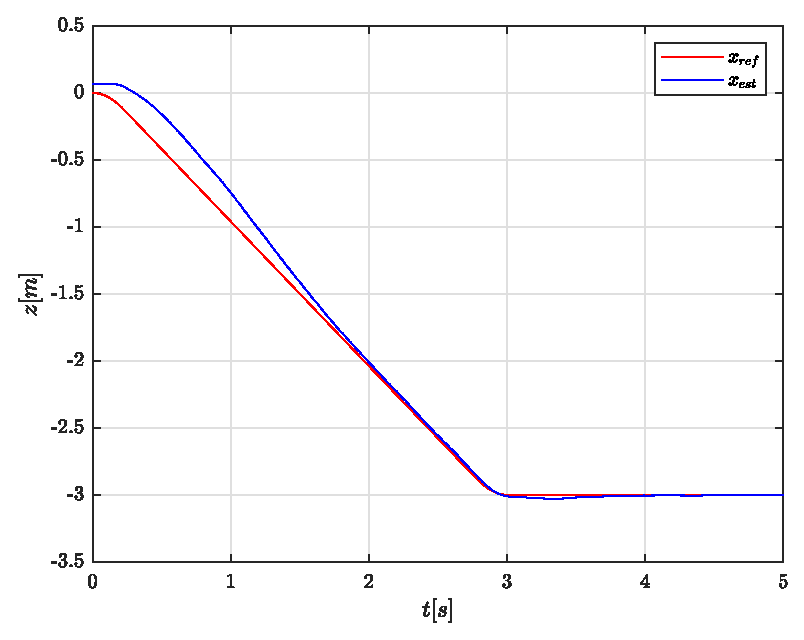
\includegraphics[width=1\textwidth]{Simulazioni/Figure/PID/STEP/AltitudeControlPos}
		\caption{Controllo posizione}
		\label{fig:STEPerrposzPID}
	\end{subfigure}
	\hfill
	\begin{subfigure}{0.45\textwidth}
		\centering
		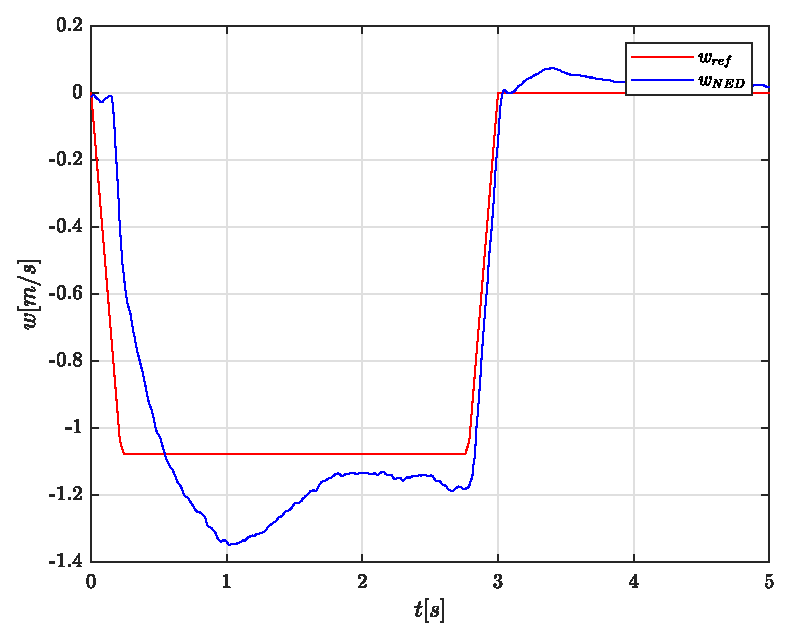
\includegraphics[width=1\textwidth]{Simulazioni/Figure/PID/STEP/AltitudeControlVel}
		\caption{Controllo velocità}
	\end{subfigure}
	\caption{Risposta del controllore PID di quota al segnale STEP}
	\label{fig:STEPerrvelzPID}
\end{figure}

\begin{figure}
	\centering
	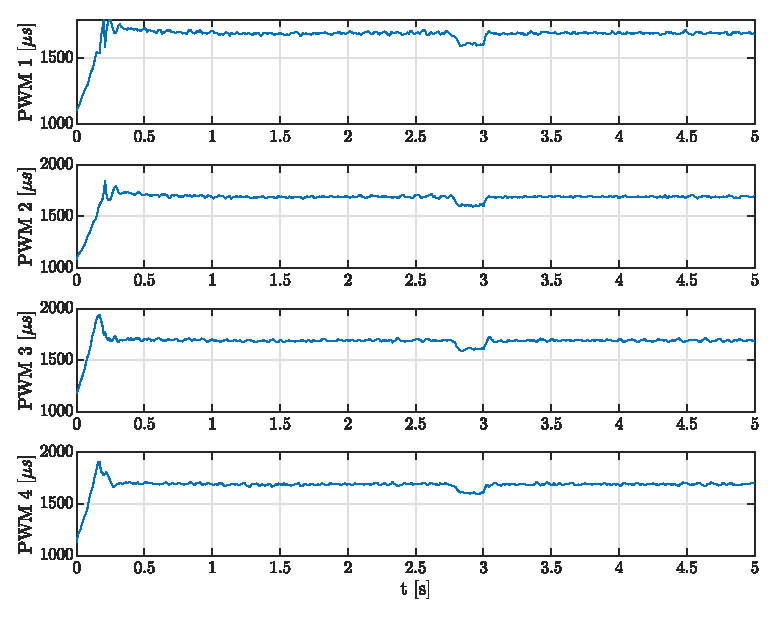
\includegraphics[width=0.5\textwidth]{Simulazioni/Figure/PID/STEP/PWM}
	\caption{Segnali PWM del controllore PID al segnale STEP}
	\label{fig:STEPerrPWMzPID}
\end{figure}

In questa simulazione si oserva come il controllore PID risponda correttamente al comando di decollo. L'errore iniziale risulta essere maggiore nella prima fase a causa dell'errore misurato inizialmente sulla quota. Nel proseguire della manovra il sistema riesce correttamente a minimizzare corettamente l'errore di posizione, Figura (\ref{fig:STEPerrposzPID}). L'inseguimento del rateo di salita risulta essere imprecisa nella fase iniziale, presentando un overshoot e un successivo assestamento lento è impreciso. Nella fase di livellamento però sia l'overshoot che l'errore stazionario si riduce, Figura (\ref{fig:STEPerrposzPID}). Il segnale PWM in uscita del controllore risulta essere abbastanza regolare, senza presentare oscillazioni eccessive, rimanendo in un range nominale e non presentando saturazione.

\subsubsection{SQUARE}

\begin{figure}
	\centering
	\begin{subfigure}{0.45\textwidth}
		\centering
		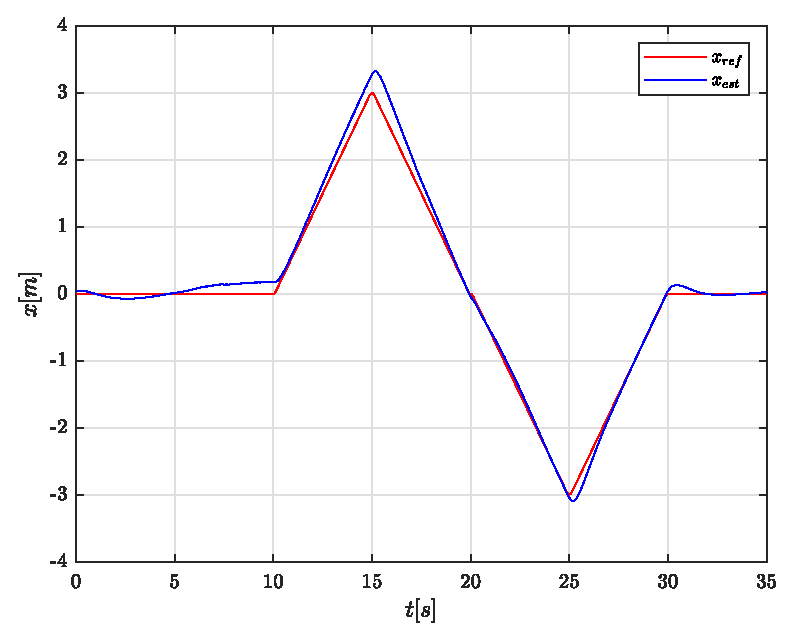
\includegraphics[width=1\textwidth]{Simulazioni/Figure/PID/SQUARE/PositionControlXPos}
		\caption{Controllo posizione lungo x}
		\label{fig:SQUAREerrposxPID}
	\end{subfigure}
	\hfill
	\begin{subfigure}{0.45\textwidth}
		\centering
		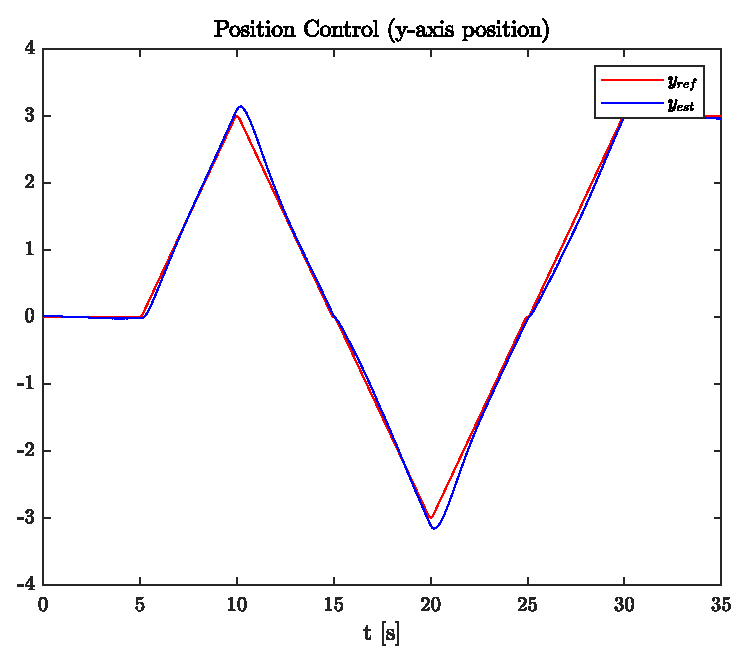
\includegraphics[width=1\textwidth]{Simulazioni/Figure/PID/SQUARE/PositionControlYPos}
		\caption{Controllo posizione lungo y}
		\label{fig:SQUAREerrposyPID}
	\end{subfigure}
	\\
	\begin{subfigure}{0.45\textwidth}
		\centering
		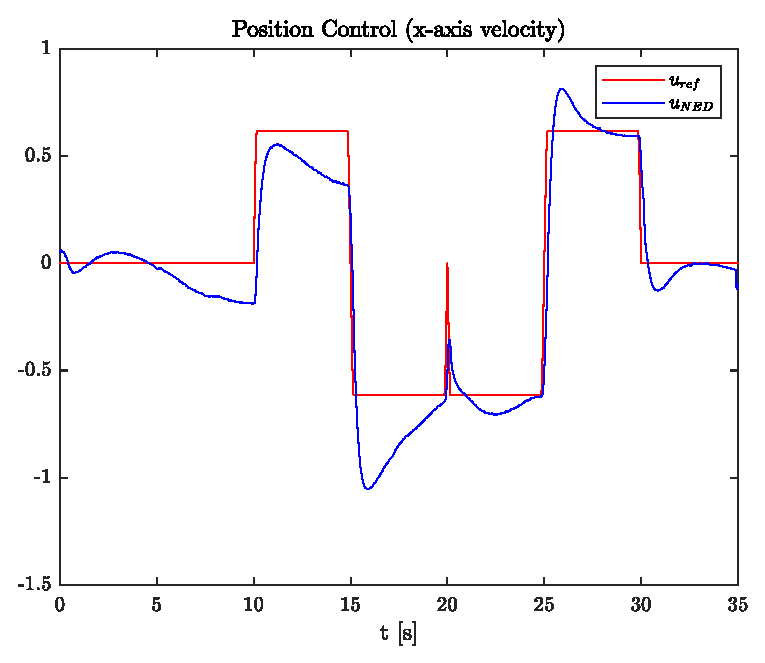
\includegraphics[width=1\textwidth]{Simulazioni/Figure/PID/SQUARE/PositionControlXVel}
		\caption{Controllo velocità lungo x}
		\label{fig:SQUAREerrvelxPID}
	\end{subfigure}
	\hfill
	\begin{subfigure}{0.45\textwidth}
		\centering
		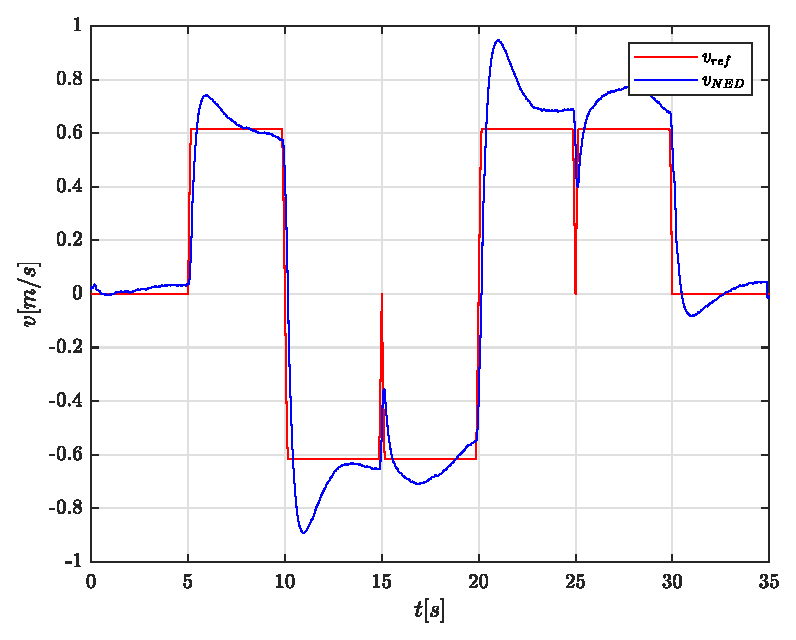
\includegraphics[width=1\textwidth]{Simulazioni/Figure/PID/SQUARE/PositionControlYVel}
		\caption{Controllo velocità lungo y}
		\label{fig:SQUAREerrvelyPID}
	\end{subfigure}
	\caption{Risposta in posizione con controllore interno PID al comando SQUARE}
\end{figure}

\begin{figure}
	\centering
	\begin{subfigure}{0.45\textwidth}
		\centering
		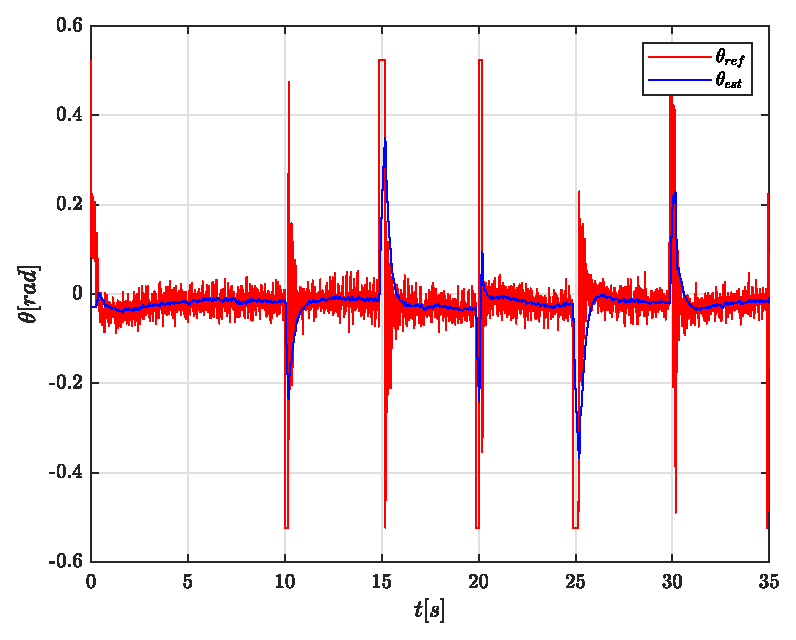
\includegraphics[width=1\textwidth]{Simulazioni/Figure/PID/SQUARE/AttitudeControlPitch}
		\caption{Controllo beccheggio}
		\label{fig:SQUAREerrbecPID}
	\end{subfigure}
	\hfill
	\begin{subfigure}{0.45\textwidth}
		\centering
		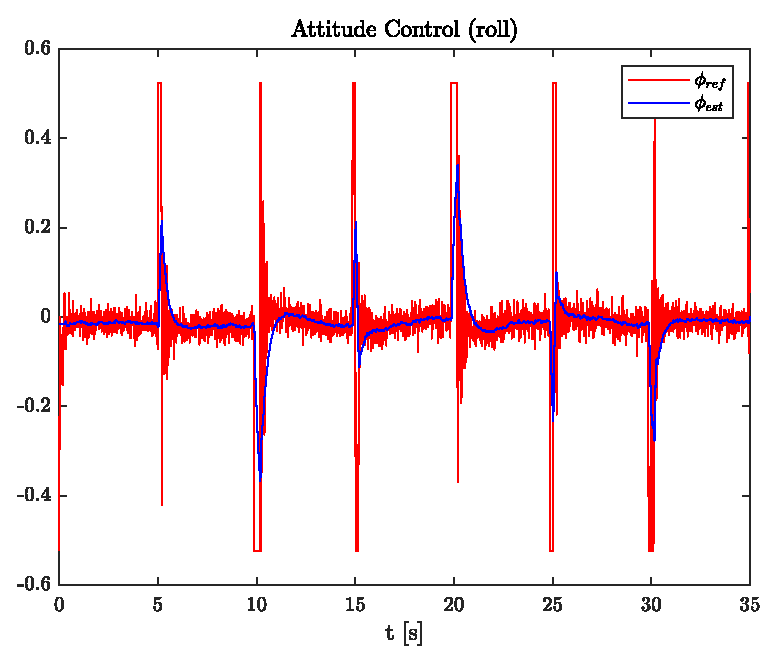
\includegraphics[width=1\textwidth]{Simulazioni/Figure/PID/SQUARE/AttitudeControlRoll}
		\caption{Controllo rollio}
		\label{fig:SQUAREerrrolPID}
	\end{subfigure}
	\hfill
	\begin{subfigure}{0.45\textwidth}
		\centering
		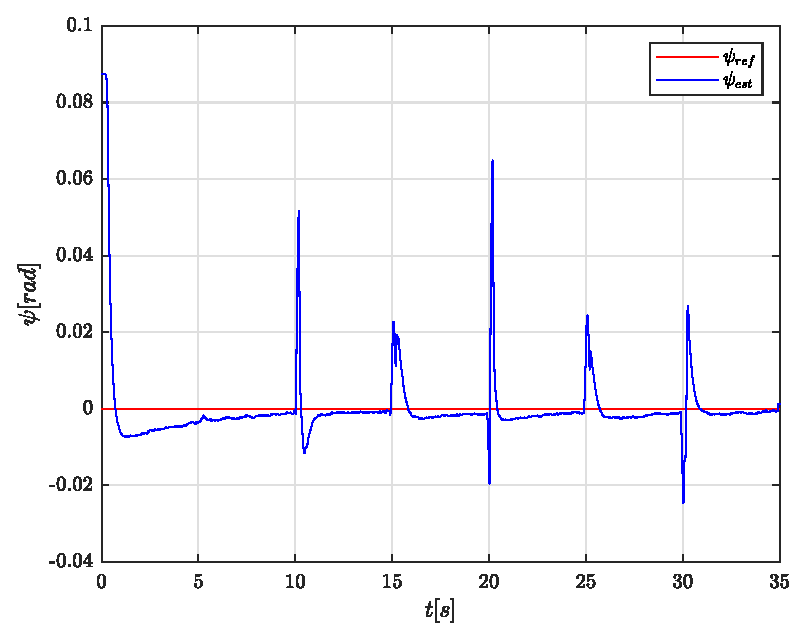
\includegraphics[width=1\textwidth]{Simulazioni/Figure/PID/SQUARE/AttitudeControlYaw}
		\caption{Controllo imbardata}
		\label{fig:SQUAREerryawPID}
	\end{subfigure}
	\caption{Risposta dell' assetto con controllore interno PID al comando SQUARE}
\end{figure}


\begin{figure}
	\centering
	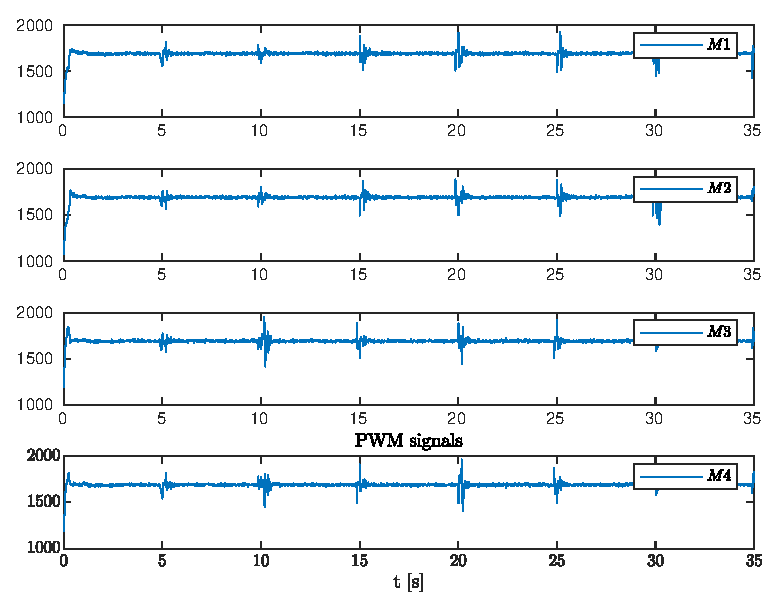
\includegraphics[width=0.5\textwidth]{Simulazioni/Figure/PID/SQUARE/PWM}
	\caption{Segnali PWM del controllore PID al segnale SQUARE}
	\label{fig:SQUAREPWMPID}
\end{figure}
\begin{figure}
	\centering
	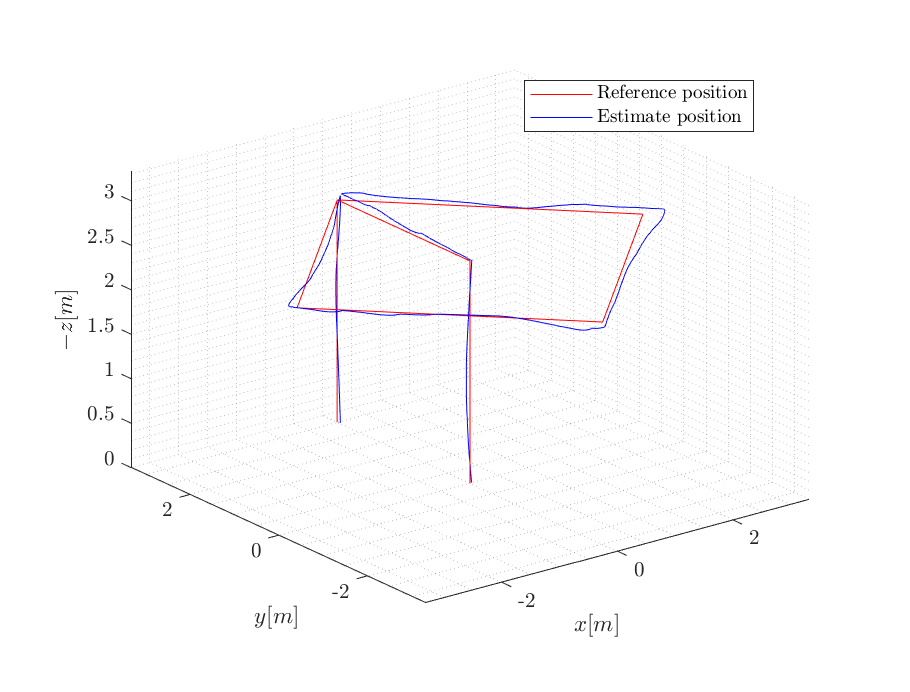
\includegraphics[width=1\textwidth]{Simulazioni/Figure/PID/SQUARE/Trajectory}
	\caption{Traiettoria percorsa con controllore PID al segnale SQUARE}
	\label{fig:SQUAREtraPID}
\end{figure}

In questa simulazione viene mostrata la capacità di muoversi nello spazio rispetto alle coordinate $x$ e $y$. L'errore di posizione osservato risulta essere relativamente piccolo. Gli incrementi di questo risultano essere maggiori nella fase di decollo iniziale e nell'attuazione dei cambi di velocità, Figure (\ref{fig:SQUAREerrposyPID}) e (\ref{fig:SQUAREerrposyPID}). L'inseguimento da parte del controllore PID nei confronti della velocità presenta alcuni picchi di overshoot quando questa subisce repentine variazioni, mostrando però l'assestamento successivo verso la riduzione asintotica della differenza. La risposta in velocità risulta essere molto rapida, Figure (\ref{fig:SQUAREerrvelyPID}) e (\ref{fig:SQUAREerrvelyPID}). Osservando i segnali di riferimento generati dal Position Control per l'Attitude Control,nelle Figure (\ref{fig:SQUAREerrbecPID}) e (\ref{fig:SQUAREerrrolPID}), si nota la presenza di intervalli in cui il controllore di posizione è in saturazione. Il segnale di riferimento generato dal Position Control presenta una componente di rumore. Il velivolo riesce comunque a seguire mediamente questo segnale, portandosi in condizione di assetto corretto per seguire la velocità di traslazione. Per quanto riguarda l'angolo di imbardata, con riferimento costante, presenta a causa degli effetti di accoppiamento tra le rotazioni lungo gli assi $x$ e $y$, degli scostamenti. Il sistema risponde molto bene per ridurre questo tipo di errore, come è osservabile nella Figura (\ref{fig:SQUAREerryawPID}). Anche in questa simulazione il segnale PWM generato è molto pulito e non presenta oscillazioni di ampiezza rilevante rispetto al valore medio, Figura (\ref{fig:SQUAREPWMPID}). Osservando la Figura (\ref{fig:SQUAREtraPID}), si osserva come il controllore sia in grado di percorrere la traiettoria prestabilita in modo efficacie, con alcune fasi di scostamento nelle variazione della direzione. La fase di atterraggio non presenta particolari criticità.

\subsubsection{BUTTERFLY}

\begin{figure}
	\centering
	\begin{subfigure}{0.45\textwidth}
		\centering
		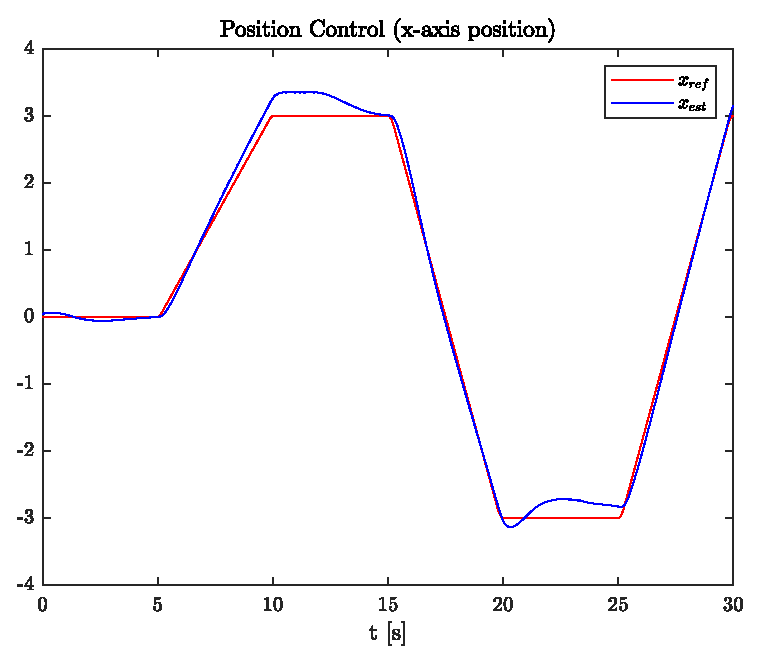
\includegraphics[width=1\textwidth]{Simulazioni/Figure/PID/BUTTERFLY/PositionControlXPos}
		\caption{Controllo posizione lungo x}
		\label{fig:BUTTERFLYerrposxPID}
	\end{subfigure}
	\hfill
	\begin{subfigure}{0.45\textwidth}
		\centering
		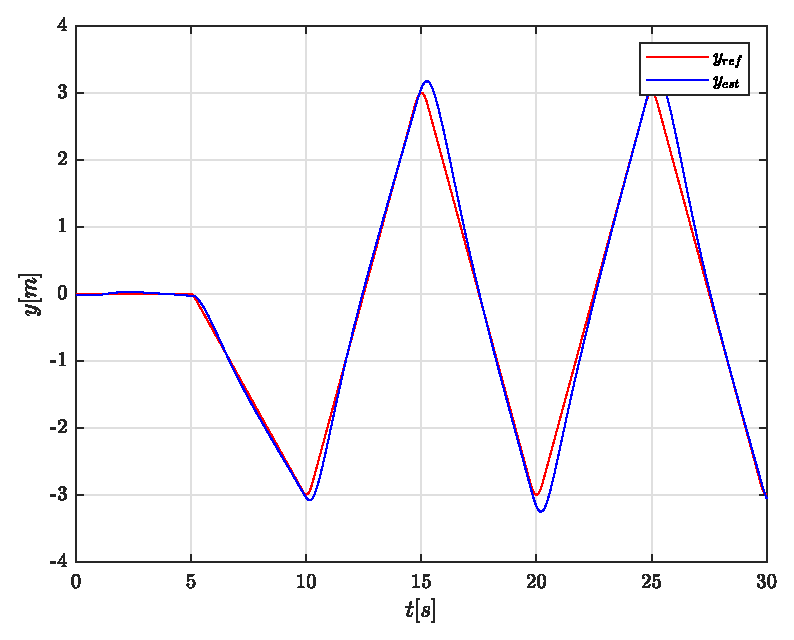
\includegraphics[width=1\textwidth]{Simulazioni/Figure/PID/BUTTERFLY/PositionControlYPos}
		\caption{Controllo posizione lungo y}
		\label{fig:BUTTERFLYerrposyPID}
	\end{subfigure}
	\\
	\begin{subfigure}{0.45\textwidth}
		\centering
		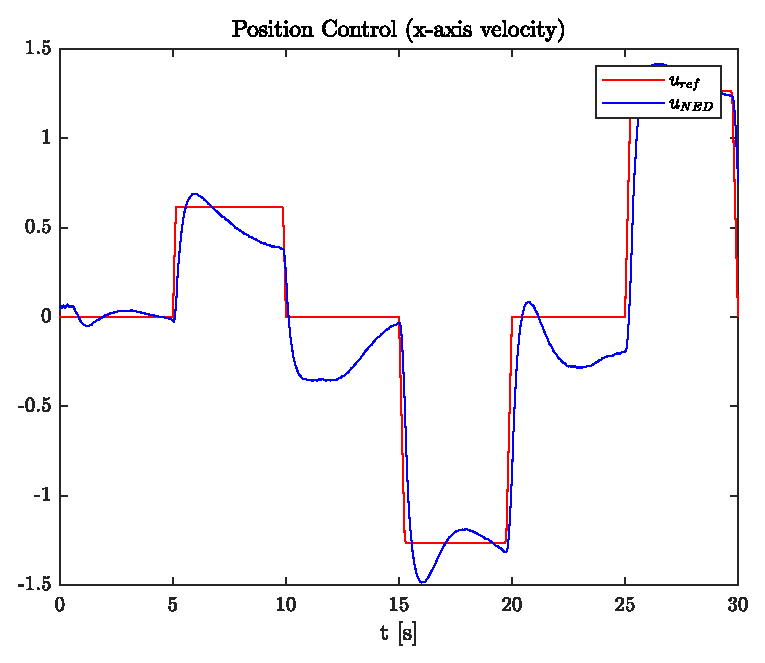
\includegraphics[width=1\textwidth]{Simulazioni/Figure/PID/BUTTERFLY/PositionControlXVel}
		\caption{Controllo velocità lungo x}
		\label{fig:BUTTERFLYerrvelxPID}
	\end{subfigure}
	\hfill
	\begin{subfigure}{0.45\textwidth}
		\centering
		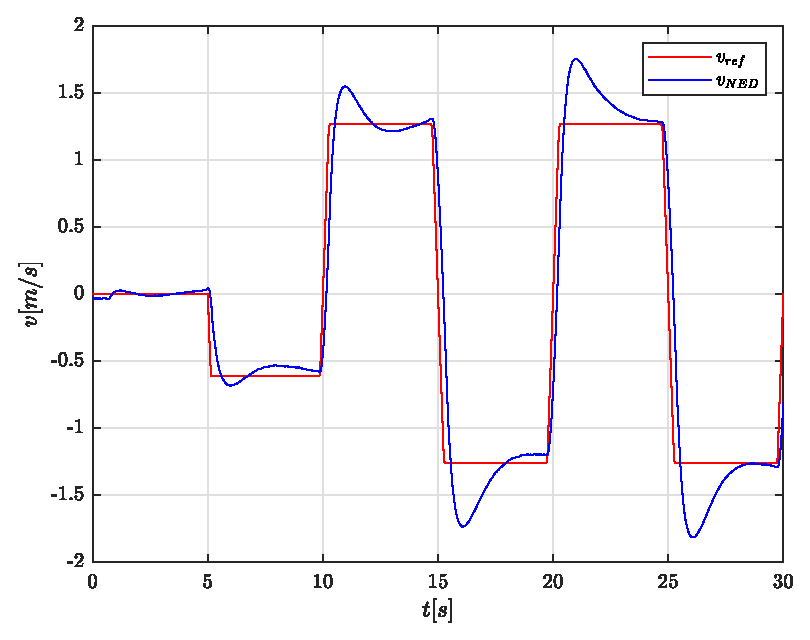
\includegraphics[width=1\textwidth]{Simulazioni/Figure/PID/BUTTERFLY/PositionControlYVel}
		\caption{Controllo velocità lungo y}
		\label{fig:BUTTERFLYerrvelyPID}
	\end{subfigure}
	\caption{Risposta in posizione con controllore interno PID al comando BUTTERFLY}
\end{figure}

\begin{figure}
	\centering
	\begin{subfigure}{0.45\textwidth}
		\centering
		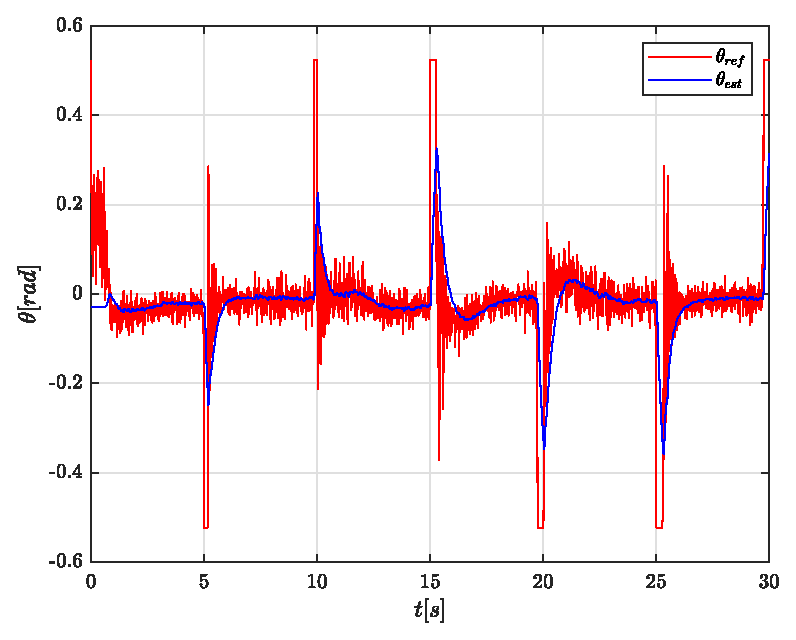
\includegraphics[width=1\textwidth]{Simulazioni/Figure/PID/BUTTERFLY/AttitudeControlPitch}
		\caption{Controllo beccheggio}
		\label{fig:BUTTERFLYerrbecPID}
	\end{subfigure}
	\hfill
	\begin{subfigure}{0.45\textwidth}
		\centering
		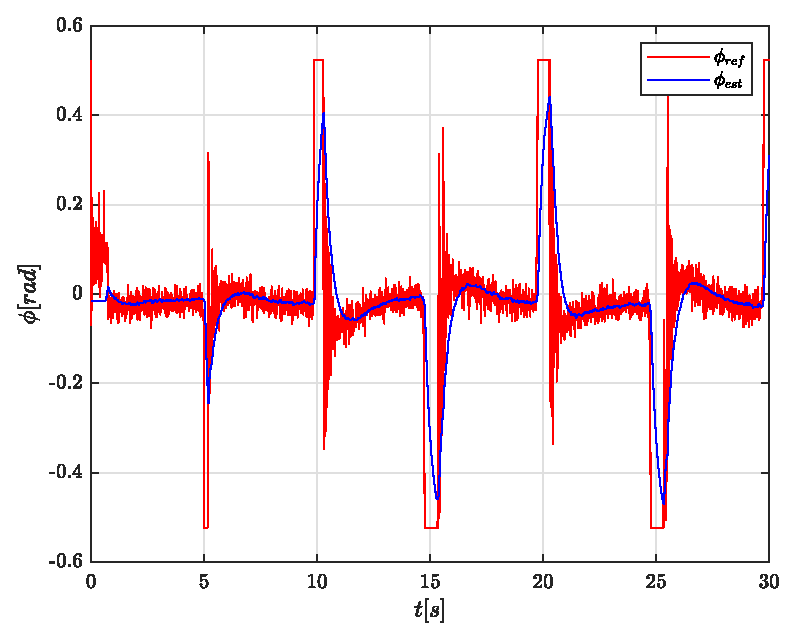
\includegraphics[width=1\textwidth]{Simulazioni/Figure/PID/BUTTERFLY/AttitudeControlRoll}
		\caption{Controllo rollio}
		\label{fig:BUTTERFLYerrrolPID}
	\end{subfigure}
	\hfill
	\begin{subfigure}{0.45\textwidth}
		\centering
		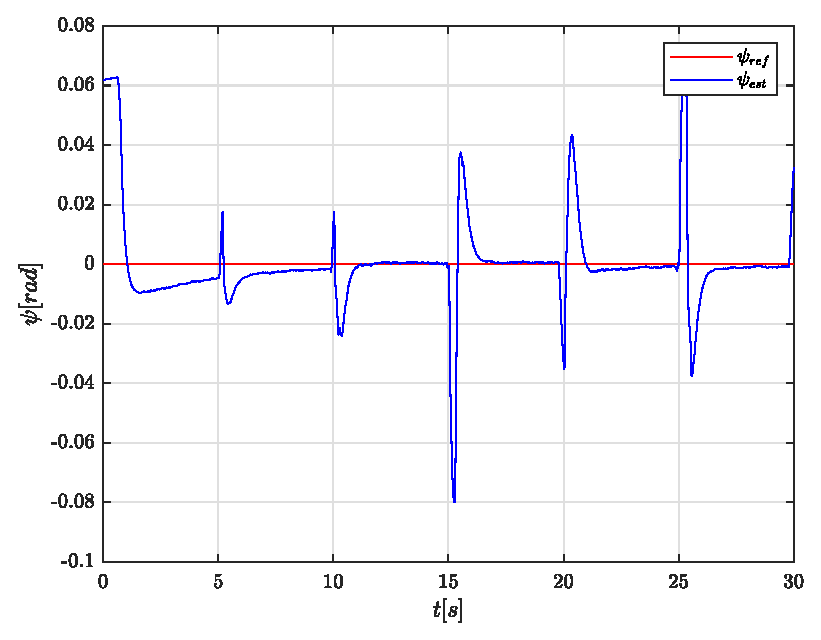
\includegraphics[width=1\textwidth]{Simulazioni/Figure/PID/BUTTERFLY/AttitudeControlYaw}
		\caption{Controllo imbardata}
		\label{fig:BUTTERFLYerryawPID}
	\end{subfigure}
	\caption{Risposta dell' assetto con controllore interno PID al comando BUTTERFLY}
\end{figure}


\begin{figure}
	\centering
	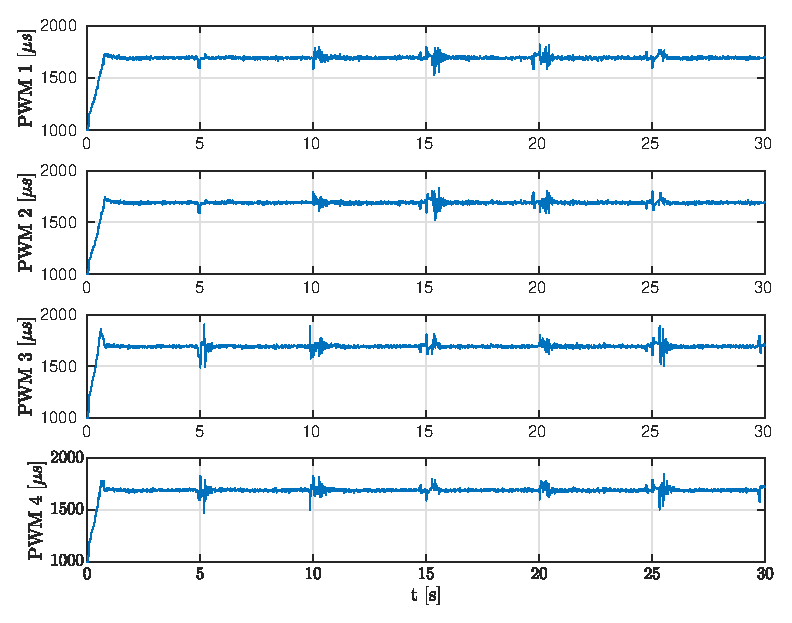
\includegraphics[width=0.5\textwidth]{Simulazioni/Figure/PID/BUTTERFLY/PWM}
	\caption{Segnali PWM del controllore PID al segnale BUTTERFLY}
	\label{fig:BUTTERFLYPWMPID}
\end{figure}
\begin{figure}
	\centering
	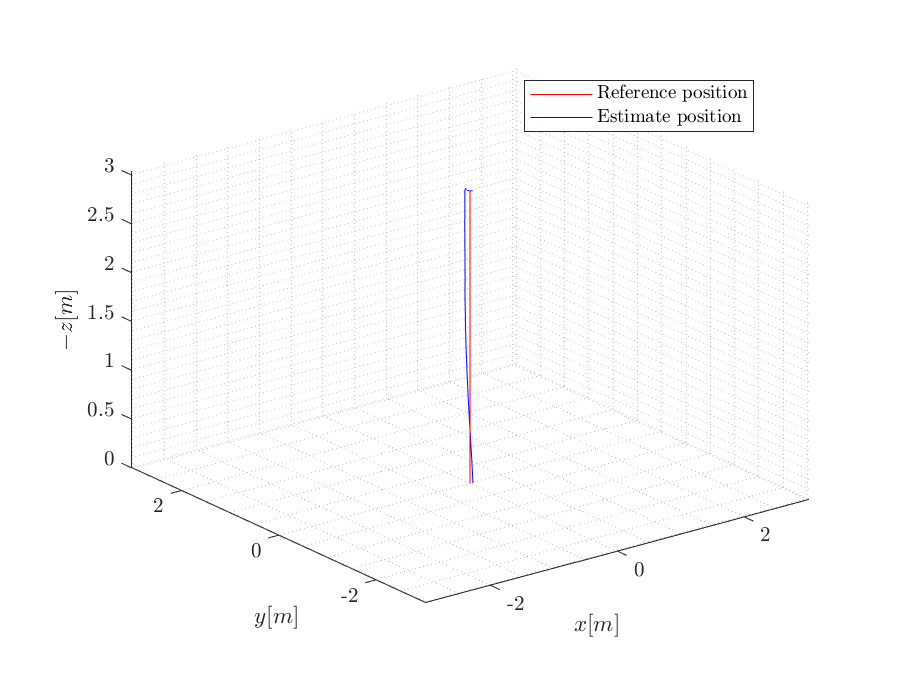
\includegraphics[width=1\textwidth]{Simulazioni/Figure/PID/BUTTERFLY/Trajectory}
	\caption{Traiettoria percorsa con controllore PID al segnale SQUARE}
	\label{fig:BUTTERFLYtraPID}
\end{figure}

In questa simulazione viene eseguito un percorso più lungo rispetto alla precedente in termine di spazio percorso, inoltre il cambiamento di direzione comandato al raggiungimento del waypoint è maggiore. La risposta è molto simile alla precedente. Anche in questa simulazione l'errore di posizione osservato risulta essere piccolo. Gli incrementi risultano maggiori nella fase di decollo iniziale e nell'attuazione dei cambi di velocità, Figure (\ref{fig:BUTTERFLYerrposyPID}) e (\ref{fig:BUTTERFLYerrposyPID}). Sono presenti i picchi di overshoot nella risposta in velocità, con una fase successiva di assestamento. La risposta in velocità è rapida, Figure (\ref{fig:BUTTERFLYerrvelyPID}) e (\ref{fig:BUTTERFLYerrvelyPID}). Nelle Figure (\ref{fig:BUTTERFLYerrbecPID}) e (\ref{fig:BUTTERFLYerrrolPID}), si nota la presenza di intervalli in cui il controllore di posizione è in saturazione e la presenza di un oscillazione rispetto ad un valore medio. Il segnale PWM generato è molto pulito e non presenta oscillazioni di ampiezza rilevante rispetto al valore medio, Figura (\ref{fig:BUTTERFLYPWMPID}). Come osservabile in Figura (\ref{fig:BUTTERFLYtraPID}), il controllore è in grado di percorrere efficacemente la traiettoria prestabilita con alcuni scostamenti in presenza di cambiamenti repentini di direzione.

\subsubsection{SNAKE}

\begin{figure}
	\centering
	\begin{subfigure}{0.45\textwidth}
		\centering
		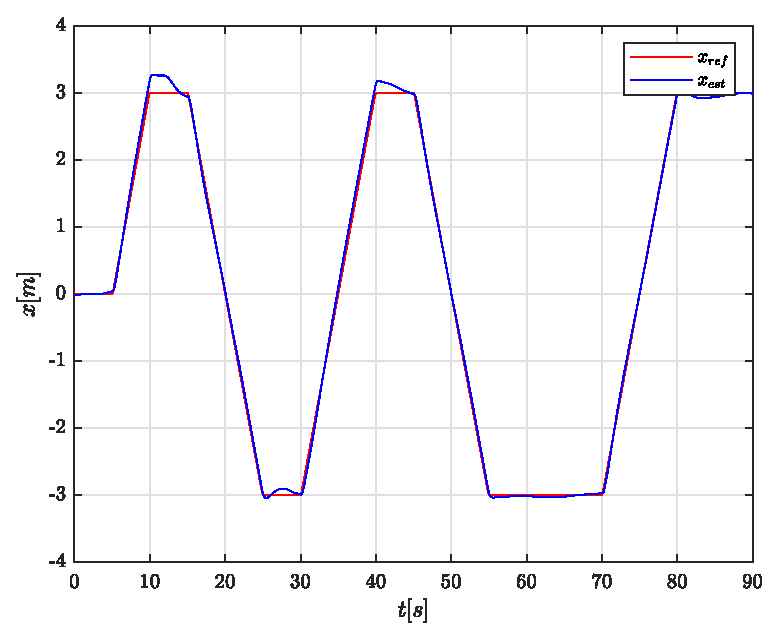
\includegraphics[width=1\textwidth]{Simulazioni/Figure/PID/SNAKE/PositionControlXPos}
		\caption{Controllo posizione lungo x}
		\label{fig:SNAKEerrposxPID}
	\end{subfigure}
	\hfill
	\begin{subfigure}{0.45\textwidth}
		\centering
		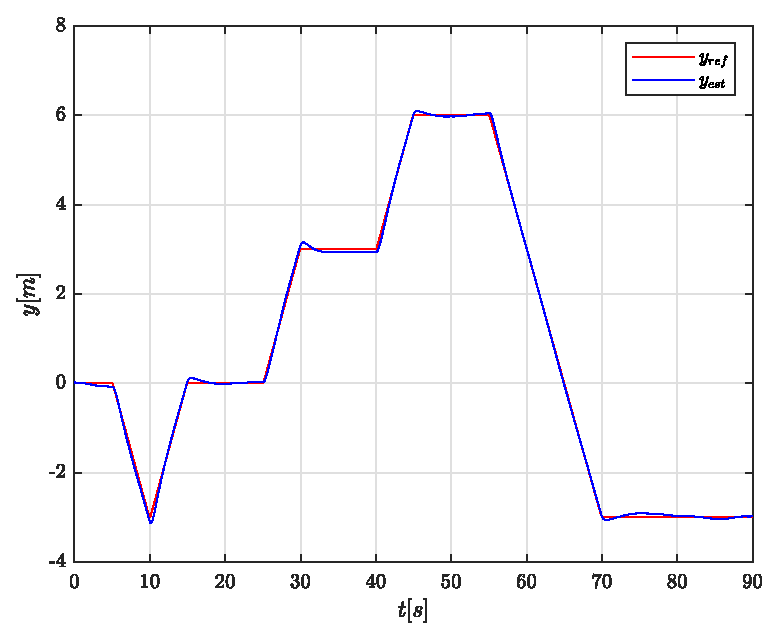
\includegraphics[width=1\textwidth]{Simulazioni/Figure/PID/SNAKE/PositionControlYPos}
		\caption{Controllo posizione lungo y}
		\label{fig:SNAKEerrposyPID}
	\end{subfigure}
	\\
	\begin{subfigure}{0.45\textwidth}
		\centering
		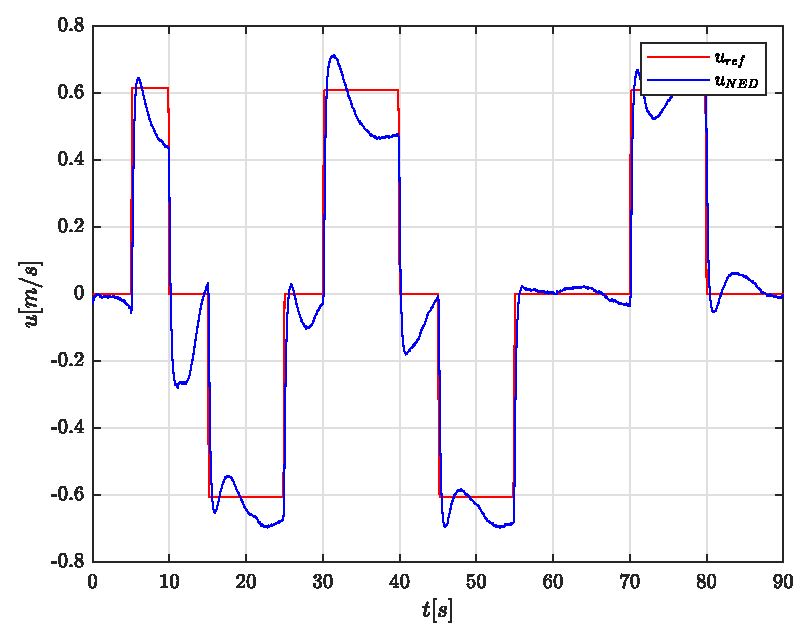
\includegraphics[width=1\textwidth]{Simulazioni/Figure/PID/SNAKE/PositionControlXVel}
		\caption{Controllo velocità lungo x}
		\label{fig:SNAKEerrvelxPID}
	\end{subfigure}
	\hfill
	\begin{subfigure}{0.45\textwidth}
		\centering
		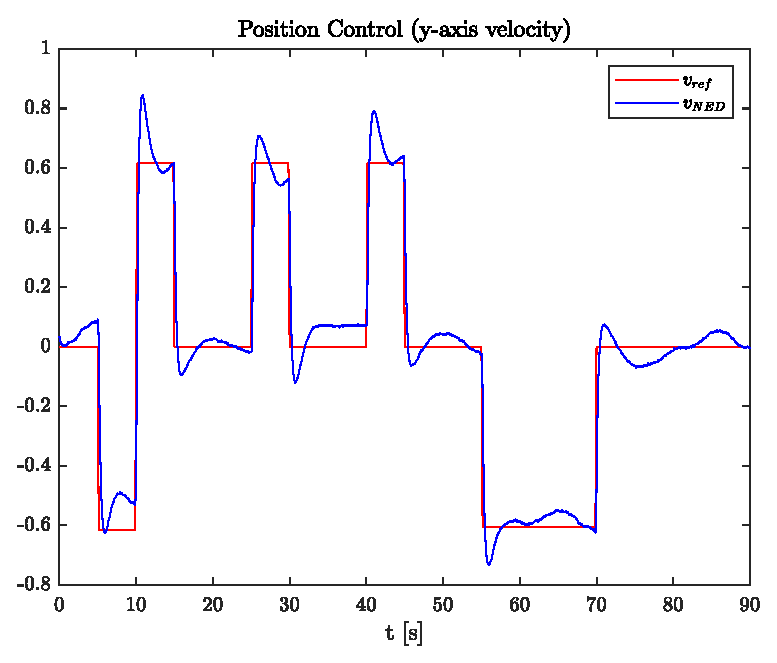
\includegraphics[width=1\textwidth]{Simulazioni/Figure/PID/SNAKE/PositionControlYVel}
		\caption{Controllo velocità lungo y}
		\label{fig:SNAKEerrvelyPID}
	\end{subfigure}
	\caption{Risposta in posizione con controllore interno PID al comando SNAKE}
\end{figure}

\begin{figure}
	\centering
	\begin{subfigure}{0.45\textwidth}
		\centering
		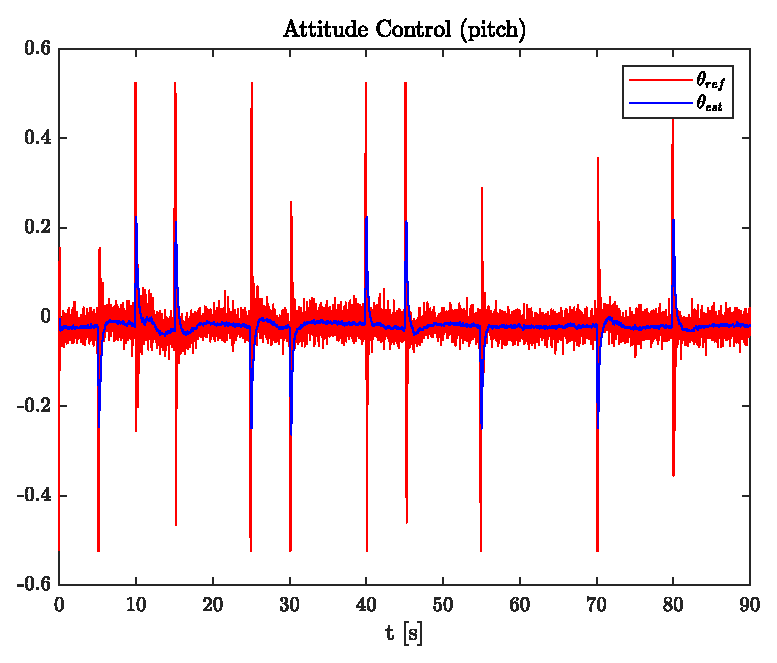
\includegraphics[width=1\textwidth]{Simulazioni/Figure/PID/SNAKE/AttitudeControlPitch}
		\caption{Controllo beccheggio}
		\label{fig:SNAKEerrbecPID}
	\end{subfigure}
	\hfill
	\begin{subfigure}{0.45\textwidth}
		\centering
		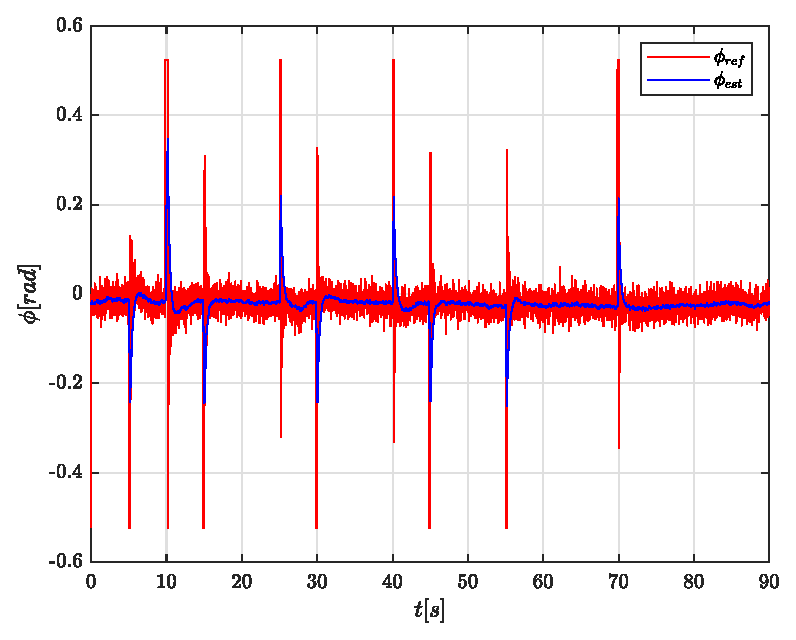
\includegraphics[width=1\textwidth]{Simulazioni/Figure/PID/SNAKE/AttitudeControlRoll}
		\caption{Controllo rollio}
		\label{fig:SNAKEerrrolPID}
	\end{subfigure}
	\hfill
	\begin{subfigure}{0.45\textwidth}
		\centering
		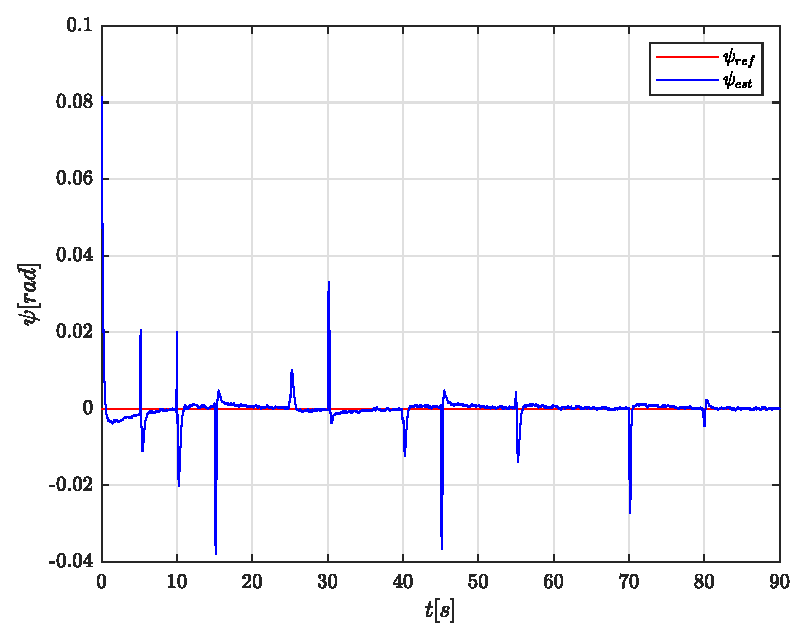
\includegraphics[width=1\textwidth]{Simulazioni/Figure/PID/SNAKE/AttitudeControlYaw}
		\caption{Controllo imbardata}
		\label{fig:SNAKEerryawPID}
	\end{subfigure}
	\caption{Risposta dell' assetto con controllore interno PID al comando SNAKE}
\end{figure}

\begin{figure}
	\centering
	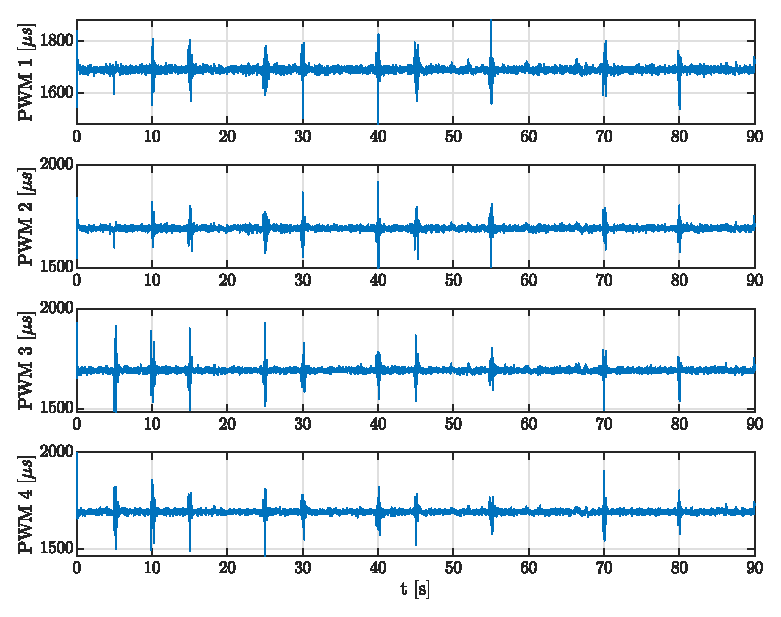
\includegraphics[width=0.5\textwidth]{Simulazioni/Figure/PID/SNAKE/PWM}
	\caption{Segnali PWM del controllore PID al segnale SNAKE}
	\label{fig:SNAKEPWMPID}
\end{figure}
\begin{figure}
	\centering
	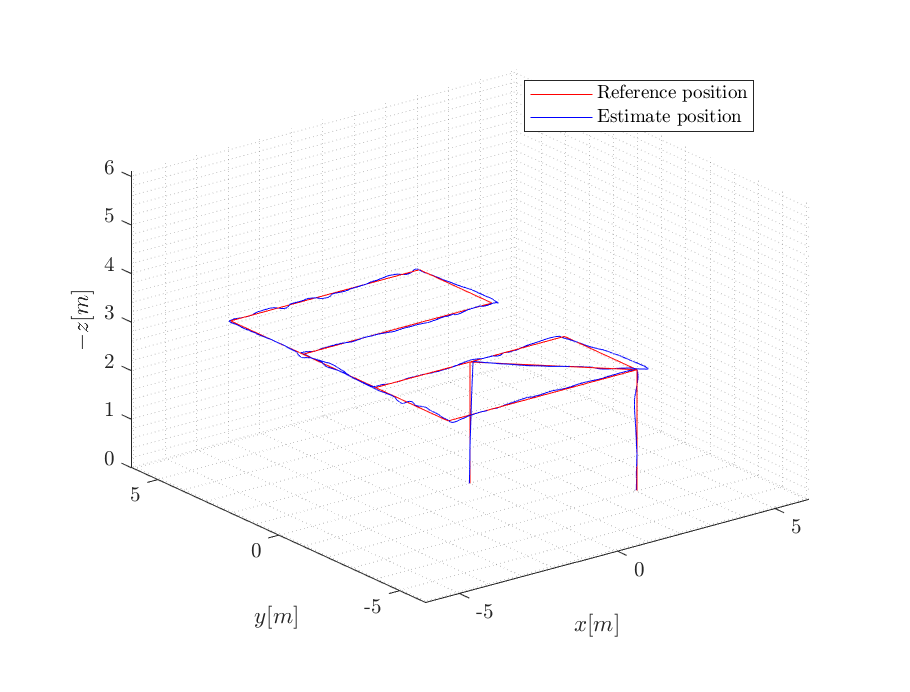
\includegraphics[width=1\textwidth]{Simulazioni/Figure/PID/SNAKE/Trajectory}
	\caption{Traiettoria percorsa con controllore PID al segnale SNAKE}
	\label{fig:SNAKEtraPID}
\end{figure}

In questa simulazione viene proposto un percorso più lungo in termine di tempo e spazio percorso. La risposta del sistema riguardante la posizione è precisa, presentando solo piccoli scostamenti nei punti in cui si ha una maggiore variazione di velocità, analogamente alle tre simulazioni mostrate in precedenza, Figure (\ref{fig:SNAKEerrposyPID}) e (\ref{fig:SNAKEerrposyPID}). Anche la risposta in termini di velocità a seguito di oscillazioni tende asintoticamente a rimanere nell'intorno del comando, Figure (\ref{fig:SNAKEerrposyPID}) e (\ref{fig:SNAKEerrposyPID}). Anche in questo caso i segnali di riferimento impartiti per gli angoli di beccheggio e rollio presentano delle situazioni di saturazione del cotnrollore di posizione e delle oscillazioni dovute alla presenza dei rumori dei sensori, Figure (\ref{fig:SNAKEerrbecPID}) e (\ref{fig:SNAKEerrrolPID}). La risposta del sistema rispetto all'angolo di imbardata è analogo alle simulazioni precedenti, Figura (\ref{fig:SNAKEerryawPID}). Il segnali PWM generati dal controllore non presentano particolari amplificazioni del rumore o saturazione, (\ref{fig:SNAKEPWMPID}). Osservando la traiettoria percorsa rispetto al riferimento, Figura (\ref{fig:SNAKEtraPID}), si nota l'efficacia del controllore con solo alcuni piccoli scostamenti.

\clearpage
\subsection{SMC}

Vengono qui riportate le simulazioni SIL utilizzando la configurazione denominata SMC nel capitolo \ref{cap:controllore}.

\subsubsection{STEP}


\begin{figure}
	\centering
	\begin{subfigure}{0.45\textwidth}
		\centering
		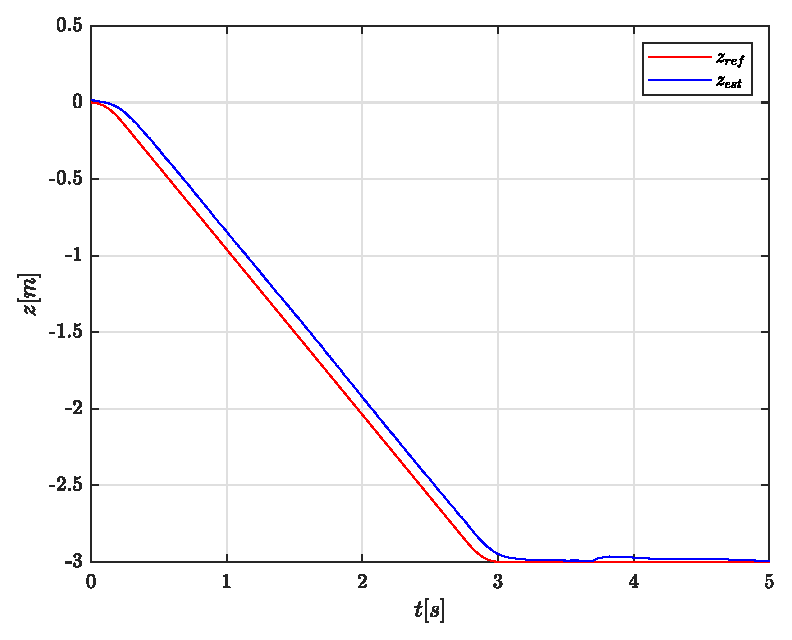
\includegraphics[width=1\textwidth]{Simulazioni/Figure/SMC/STEP/AltitudeControlPos}
		\caption{Controllo posizione}
		\label{fig:STEPerrposzSMC}
	\end{subfigure}
	\hfill
	\begin{subfigure}{0.45\textwidth}
		\centering
		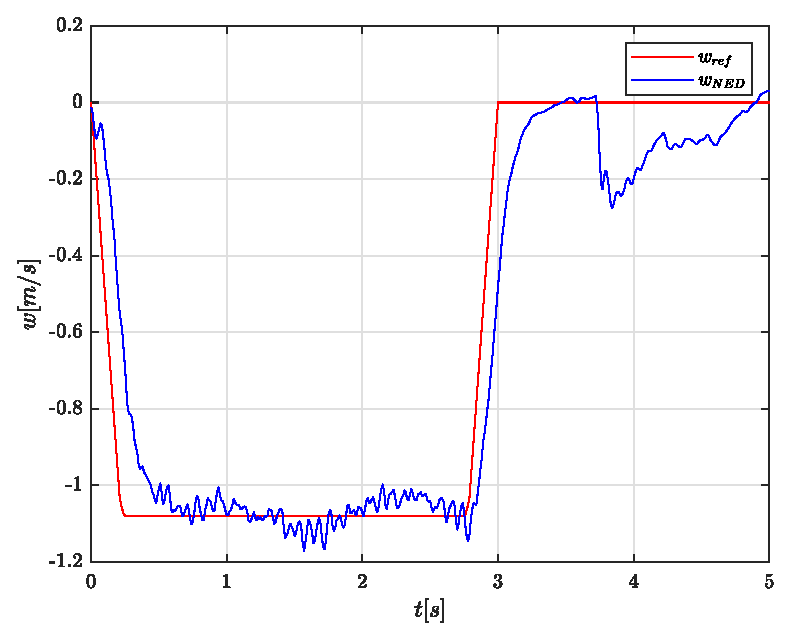
\includegraphics[width=1\textwidth]{Simulazioni/Figure/SMC/STEP/AltitudeControlVel}
		\caption{Controllo velocità}
		\label{fig:STEPerrvelzSMC}
	\end{subfigure}
	\caption{Risposta del controllore SMC di quota al segnale STEP}	
\end{figure}

\begin{figure}
	\centering
	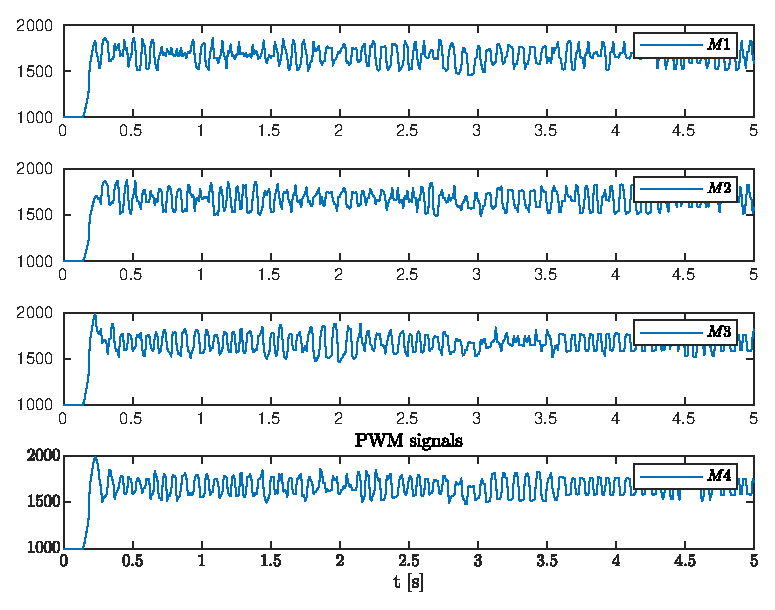
\includegraphics[width=0.5\textwidth]{Simulazioni/Figure/SMC/STEP/PWM}
	\caption{Segnali PWM generati del controllore SMC al segnale STEP}
	\label{fig:STEPPWMSMC}
\end{figure}

La risposta del controllore SMC in merito alla posizione è abbastanza precisa. Sussiste una differenza piccola ma costante lungo tutta la salita, differenza che si annulla rapidamente a livellamento, Figura (\ref{fig:STEPerrposzSMC}). Il profilo di velocità è seguito anch'esso con abbastanza precisione, esiste in questo caso un oscillazione costante nella risposta in velocità rispetto al valore di riferimento della velocità, Figura (\ref{fig:STEPerrvelzSMC}). Il segnale PWM generato da controllore mostra un comportamento discontinuo con ampiezza molto marcata, Figura (\ref{fig:STEPPWMSMC}).

\subsubsection{SQUARE}
\begin{figure}
	\centering
	\begin{subfigure}{0.45\textwidth}
		\centering
		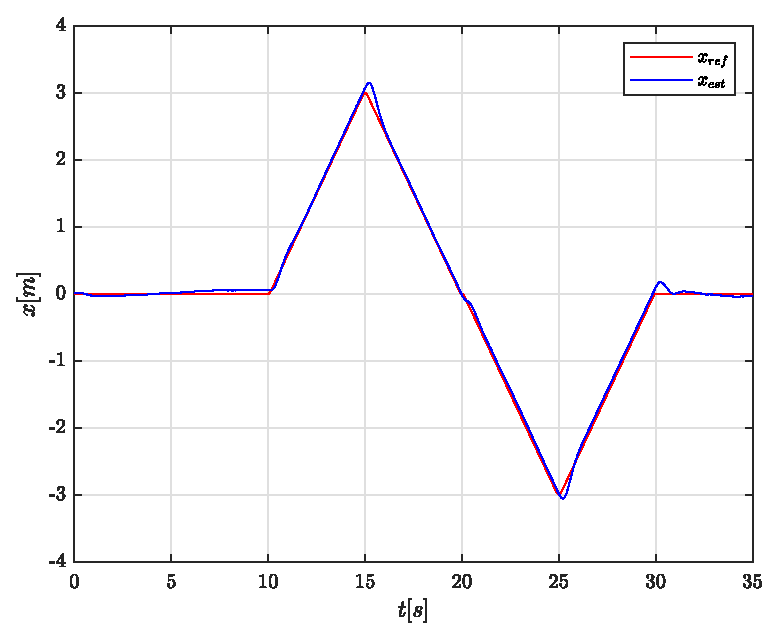
\includegraphics[width=1\textwidth]{Simulazioni/Figure/SMC/SQUARE/PositionControlXPos}
		\caption{Controllo posizione lungo x}
		\label{fig:SQUAREerrposxSMC}
	\end{subfigure}
	\hfill
	\begin{subfigure}{0.45\textwidth}
		\centering
		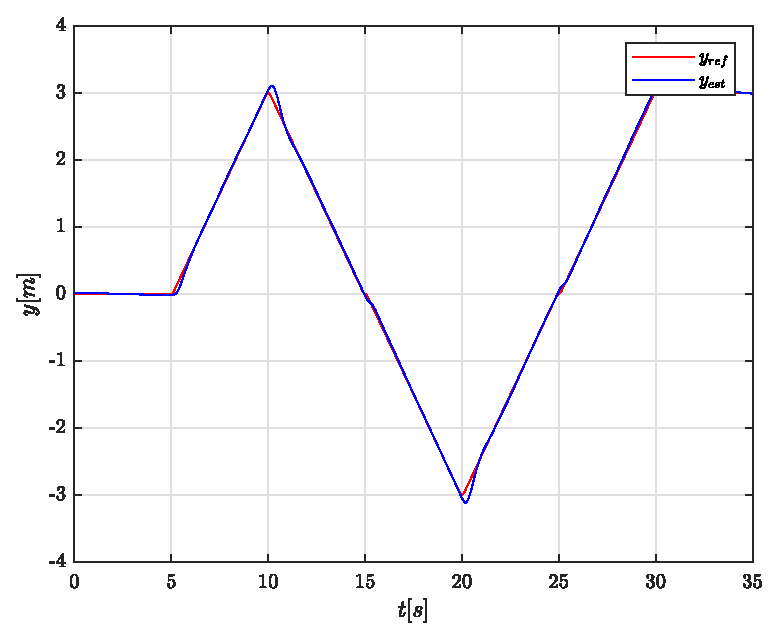
\includegraphics[width=1\textwidth]{Simulazioni/Figure/SMC/SQUARE/PositionControlYPos}
		\caption{Controllo posizione lungo y}
		\label{fig:SQUAREerrposySMC}
	\end{subfigure}
	\\
	\begin{subfigure}{0.45\textwidth}
		\centering
		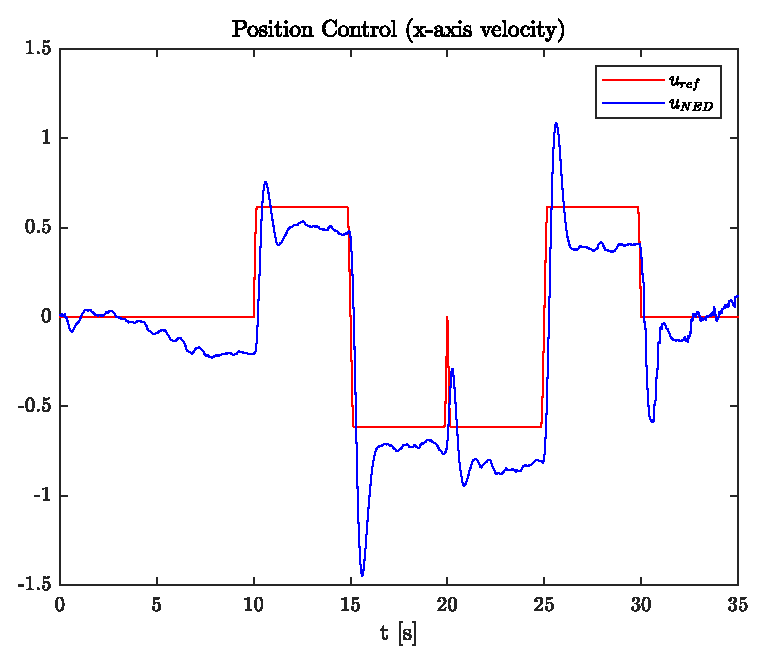
\includegraphics[width=1\textwidth]{Simulazioni/Figure/SMC/SQUARE/PositionControlXVel}
		\caption{Controllo velocità lungo x}
		\label{fig:SQUAREerrvelxSMC}
	\end{subfigure}
	\hfill
	\begin{subfigure}{0.45\textwidth}
		\centering
		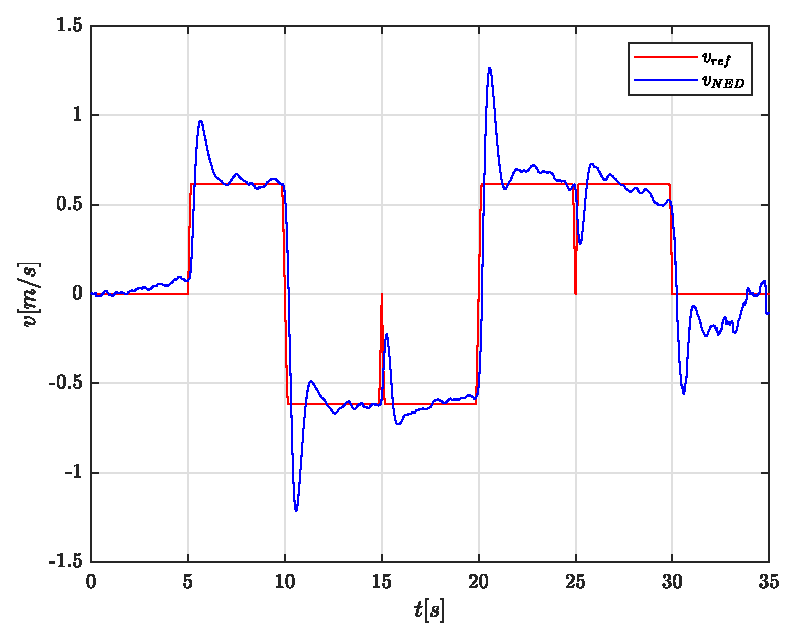
\includegraphics[width=1\textwidth]{Simulazioni/Figure/SMC/SQUARE/PositionControlYVel}
		\caption{Controllo velocità lungo y}
		\label{fig:SQUAREerrvelySMC}
	\end{subfigure}
	\caption{Risposta del controllo posizione con controllore SMC al comando SQUARE}
\end{figure}

\begin{figure}
	\centering
	\begin{subfigure}{0.45\textwidth}
		\centering
		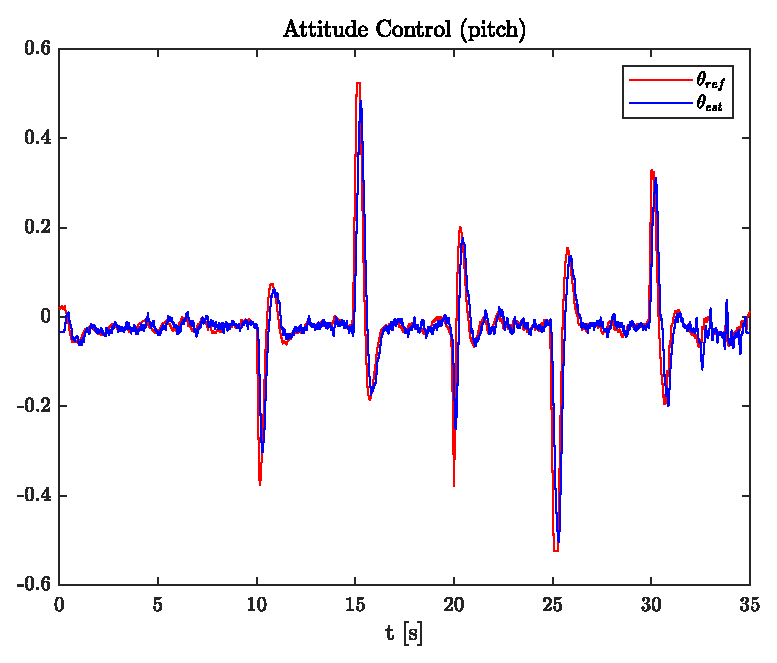
\includegraphics[width=1\textwidth]{Simulazioni/Figure/SMC/SQUARE/AttitudeControlPitch}
		\caption{Controllo beccheggio}
		\label{fig:SQUAREbecSMC}
	\end{subfigure}
	\hfill
	\begin{subfigure}{0.45\textwidth}
		\centering
		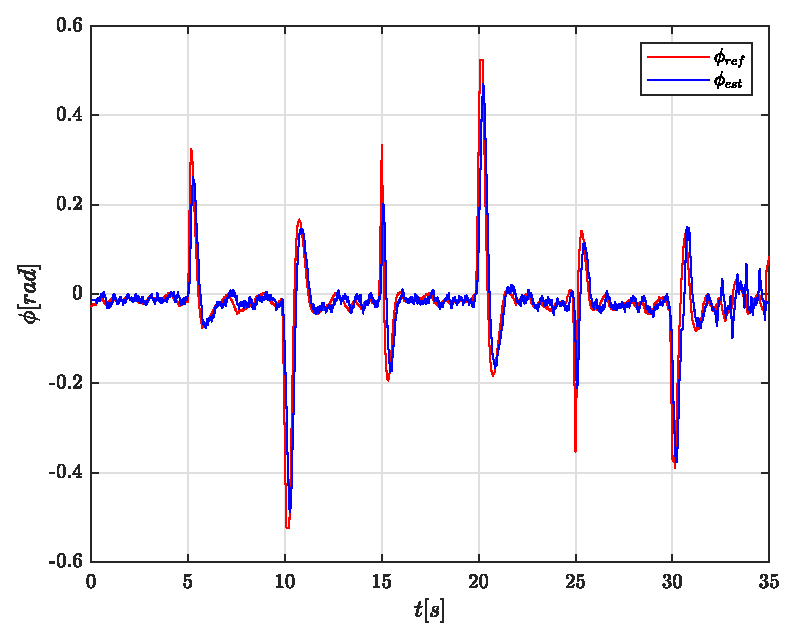
\includegraphics[width=1\textwidth]{Simulazioni/Figure/SMC/SQUARE/AttitudeControlRoll}
		\caption{Controllo rollio}
		\label{fig:SQUARErolSMC}
	\end{subfigure}
	\hfill
	\begin{subfigure}{0.45\textwidth}
		\centering
		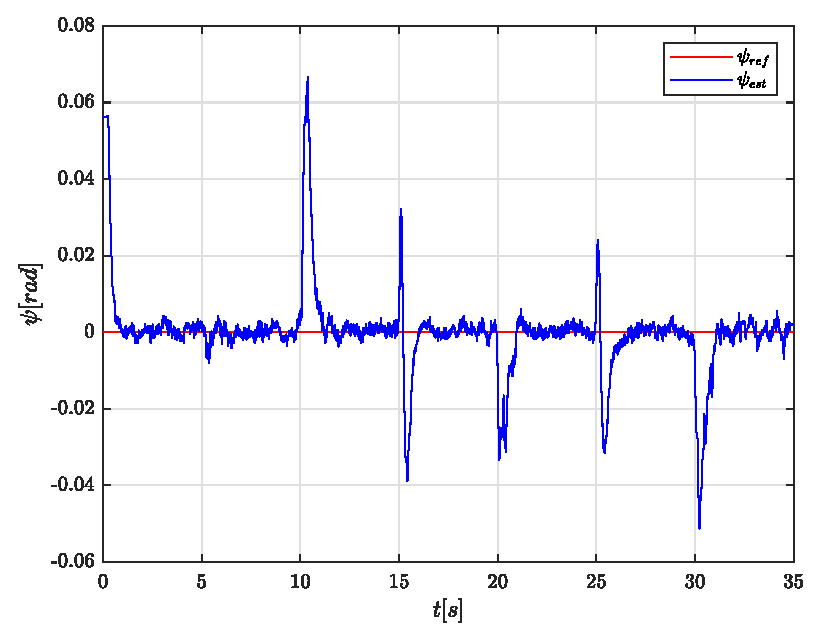
\includegraphics[width=1\textwidth]{Simulazioni/Figure/SMC/SQUARE/AttitudeControlYaw}
		\caption{Controllo imbardata}
		\label{fig:SQUAREyawSMC}
	\end{subfigure}
	\caption{Risposta dell' assetto con controllore interno SMC al comando SQUARE}
\end{figure}


\begin{figure}
	\centering
	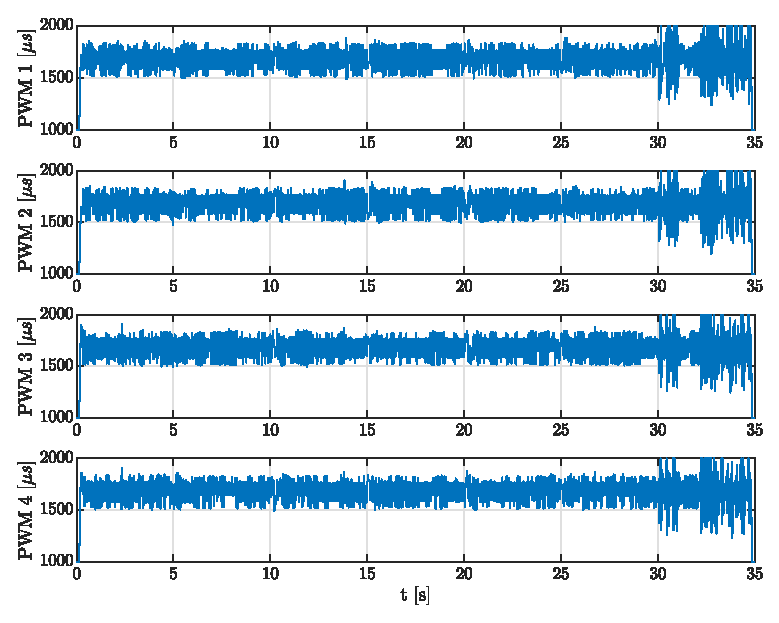
\includegraphics[width=0.5\textwidth]{Simulazioni/Figure/SMC/SQUARE/PWM}
	\caption{Segnali PWM del controllore SMC al segnale SQUARE}
	\label{fig:SQUAREPWMSMC}
\end{figure}
\begin{figure}
	\centering
	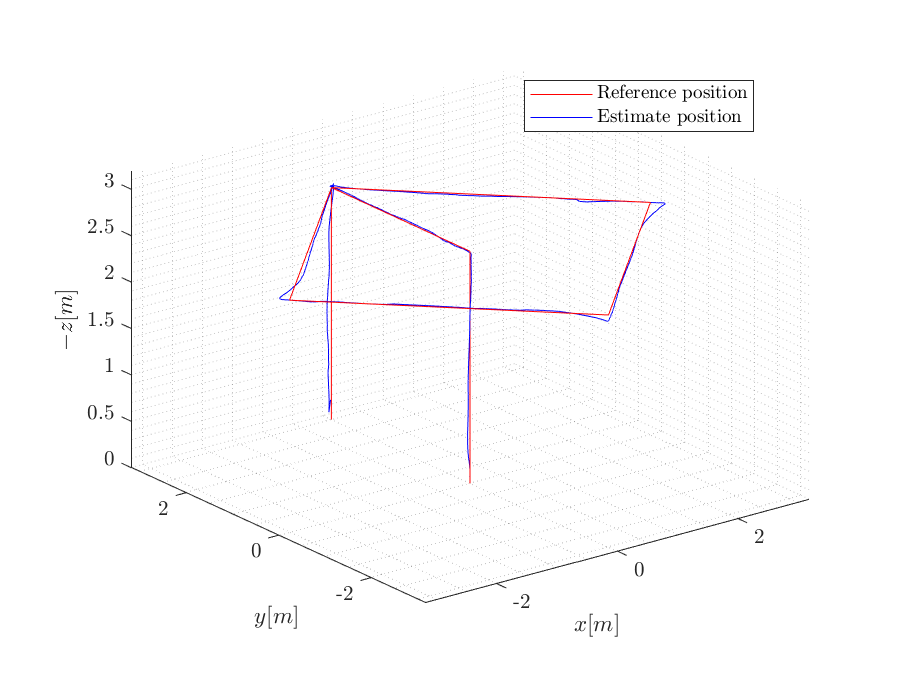
\includegraphics[width=1\textwidth]{Simulazioni/Figure/SMC/SQUARE/Trajectory}
	\caption{Traiettoria percorsa con controllore SMC al segnale SQUARE}
	\label{fig:SQUAREtraSMC}
\end{figure}

\todo{Da cambiare}
In questa simulazione viene mostrata la capacità di muoversi nello spazio rispetto alle coordinate $x$ e $y$. L'errore di posizione osservato risulta essere relativamente piccolo. Gli incrementi di questo risultano essere maggiori nella fase di decollo iniziale e nell'attuazione dei cambi di velocità, Figure (\ref{fig:SQUAREerrposyPID}) e (\ref{fig:SQUAREerrposyPID}). L'inseguimento da parte del controllore PID nei confronti della velocità presenta alcuni picchi di overshoot quando questa subisce repentine variazioni, mostrando però l'assestamento successivo verso la riduzione asintotica della differenza. La risposta in velocità risulta essere molto rapida, Figure (\ref{fig:SQUAREerrvelyPID}) e (\ref{fig:SQUAREerrvelyPID}). Osservando i segnali di riferimento generati dal Position Control per l'Attitude Control,nelle Figure (\ref{fig:SQUAREerrbecPID}) e (\ref{fig:SQUAREerrrolPID}), si nota la presenza di intervalli in cui il controllore di posizione è in saturazione. Il segnale di riferimento generato dal Position Control presenta una componente di rumore. Il velivolo riesce comunque a seguire mediamente questo segnale, portandosi in condizione di assetto corretto per seguire la velocità di traslazione. Per quanto riguarda l'angolo di imbardata, con riferimento costante, presenta a causa degli effetti di accoppiamento tra le rotazioni lungo gli assi $x$ e $y$, degli scostamenti. Il sistema risponde molto bene per ridurre questo tipo di errore, come è osservabile nella Figura (\ref{fig:SQUAREerryawPID}). Anche in questa simulazione il segnale PWM generato è molto pulito e non presenta oscillazioni di ampiezza rilevante rispetto al valore medio, Figura (\ref{fig:SQUAREPWMPID}). Osservando la Figura (\ref{fig:SQUAREtraPID}), si osserva come il controllore sia in grado di percorrere la traiettoria prestabilita in modo efficacie, con alcune fasi di scostamento nelle variazione della direzione. La fase di atterraggio non presenta particolari criticità.


\subsubsection{BUTTERFLY}

\begin{figure}
	\centering
	\begin{subfigure}{0.45\textwidth}
		\centering
		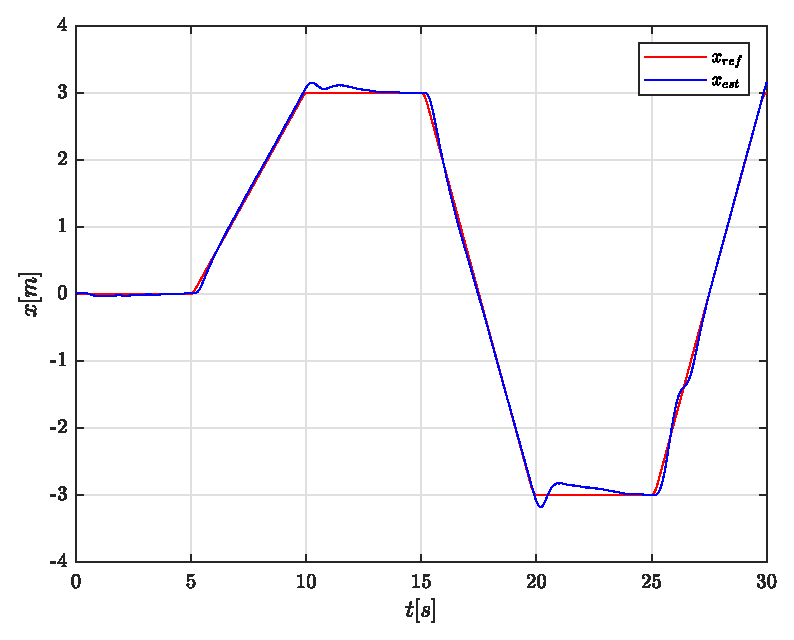
\includegraphics[width=1\textwidth]{Simulazioni/Figure/SMC/BUTTERFLY/PositionControlXPos}
		\caption{Controllo posizione lungo x}
		\label{fig:BUTTERFLYerrposxSMC}
	\end{subfigure}
	\hfill
	\begin{subfigure}{0.45\textwidth}
		\centering
		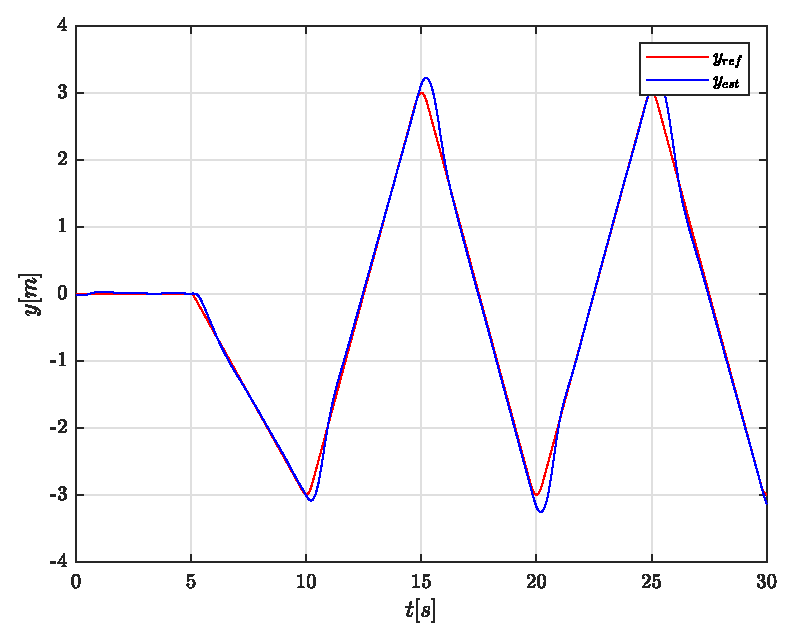
\includegraphics[width=1\textwidth]{Simulazioni/Figure/SMC/BUTTERFLY/PositionControlYPos}
		\caption{Controllo posizione lungo y}
		\label{fig:BUTTERFLYerrposySMC}
	\end{subfigure}
	\\
	\begin{subfigure}{0.45\textwidth}
		\centering
		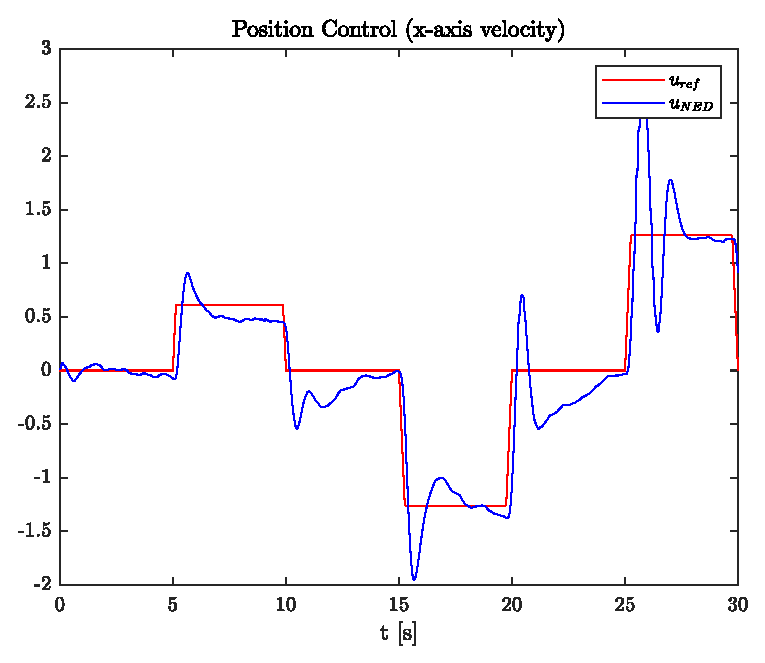
\includegraphics[width=1\textwidth]{Simulazioni/Figure/SMC/BUTTERFLY/PositionControlXVel}
		\caption{Controllo velocità lungo x}
		\label{fig:BUTTERFLYerrvelxSMC}
	\end{subfigure}
	\hfill
	\begin{subfigure}{0.45\textwidth}
		\centering
		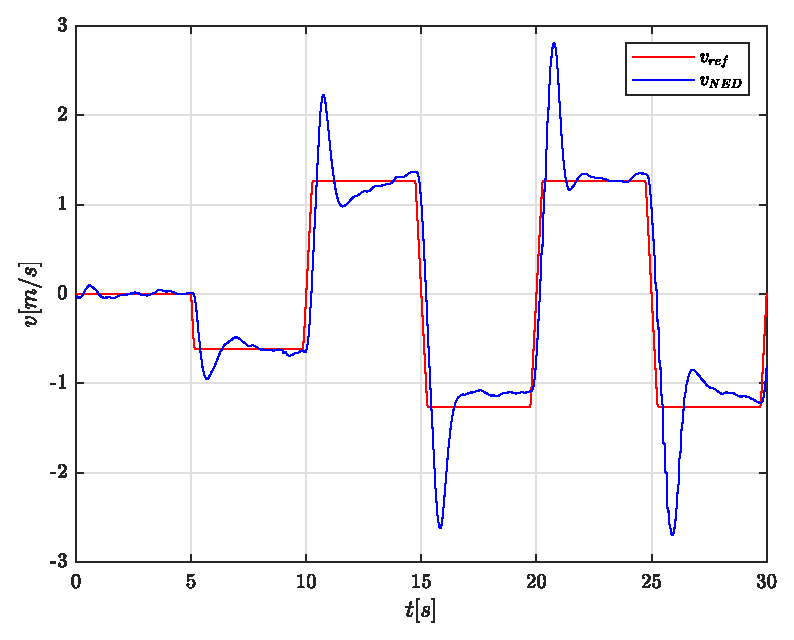
\includegraphics[width=1\textwidth]{Simulazioni/Figure/SMC/BUTTERFLY/PositionControlYVel}
		\caption{Controllo velocità lungo y}
		\label{fig:BUTTERFLYerrvelySMC}
	\end{subfigure}
	\caption{Risposta in posizione con controllore interno SMC al comando BUTTERFLY}
\end{figure}

\begin{figure}
	\centering
	\begin{subfigure}{0.45\textwidth}
		\centering
		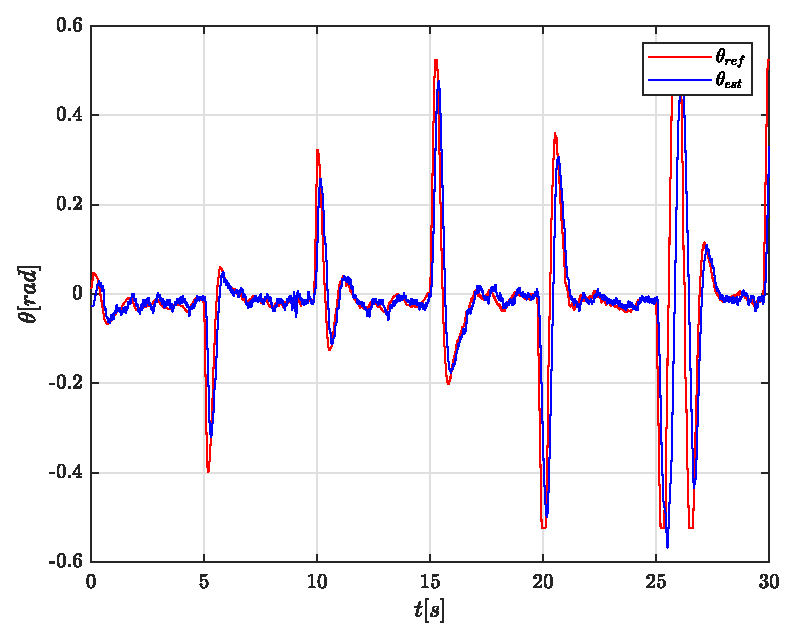
\includegraphics[width=1\textwidth]{Simulazioni/Figure/SMC/BUTTERFLY/AttitudeControlPitch}
		\caption{Controllo beccheggio}
		\label{fig:BUTTERFLYbecSMC}
	\end{subfigure}
	\hfill
	\begin{subfigure}{0.45\textwidth}
		\centering
		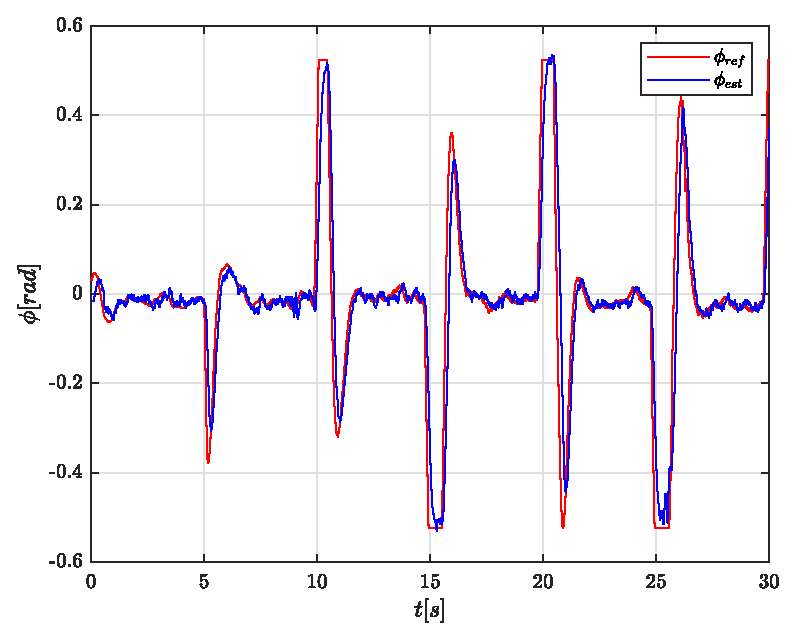
\includegraphics[width=1\textwidth]{Simulazioni/Figure/SMC/BUTTERFLY/AttitudeControlRoll}
		\caption{Controllo rollio}
		\label{fig:BUTTERFLYrolSMC}
	\end{subfigure}
	\hfill
	\begin{subfigure}{0.45\textwidth}
		\centering
		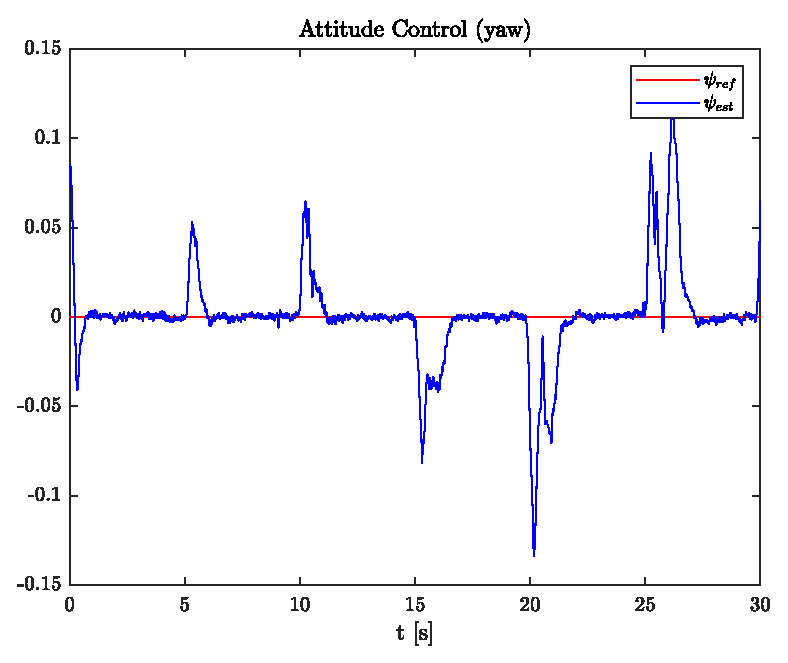
\includegraphics[width=1\textwidth]{Simulazioni/Figure/SMC/BUTTERFLY/AttitudeControlYaw}
		\caption{Controllo imbardata}
		\label{fig:BUTTERFLYyawSMC}
	\end{subfigure}
	\caption{Risposta dell' assetto con controllore interno SMC al comando BUTTERFLY}
\end{figure}

\begin{figure}
	\centering
	\includegraphics[width=0.5\textwidth]{Simulazioni/Figure/SMC/BUTTERFLY/PWM}
	\caption{Segnali PWM del controllore SMC al segnale BUTTERFLY}
	\label{fig:BUTTERFLYPWMSMC}
\end{figure}
\begin{figure}
	\centering
	\includegraphics[width=1\textwidth]{Simulazioni/Figure/SMC/BUTTERFLY/Trajectory}
	\caption{Traiettoria percorsa con controllore SMC al segnale BUTTERFLY}
	\label{fig:BUTTERFLYtraSMC}
\end{figure}

\todo{Da cambiare}
In questa simulazione si oserva come il controllore PID risponda correttamente al comando di decollo. L'errore iniziale risulta essere maggiore nella prima fase a causa dell'errore misurato inizialmente sulla quota. Nel proseguire della manovra il sistema riesce correttamente a minimizzare corettamente l'errore di posizione, Figura (\ref{fig:STEPerrposzPID}). L'inseguimento del rateo di salita risulta essere imprecisa nella fase iniziale, presentando un overshoot e un successivo assestamento lento è impreciso. Nella fase di livellamento però sia l'overshoot che l'errore stazionario si riduce, Figura (\ref{fig:STEPerrposzPID}). Il segnale PWM in uscita del controllore risulta essere abbastanza regolare, senza presentare oscillazioni eccessive, rimanendo in un range nominale e non presentando saturazione.

\subsubsection{SNAKE}
\begin{figure}
	\centering
	\begin{subfigure}{0.45\textwidth}
		\centering
		\includegraphics[width=1\textwidth]{Simulazioni/Figure/SMC/SNAKE/PositionControlXPos}
		\caption{Controllo posizione lungo x}
		\label{fig:SNAKEerrposxSMC}
	\end{subfigure}
	\hfill
	\begin{subfigure}{0.45\textwidth}
		\centering
		\includegraphics[width=1\textwidth]{Simulazioni/Figure/SMC/SNAKE/PositionControlYPos}
		\caption{Controllo posizione lungo y}
		\label{fig:SNAKEerrposySMC}
	\end{subfigure}
	\\
	\begin{subfigure}{0.45\textwidth}
		\centering
		\includegraphics[width=1\textwidth]{Simulazioni/Figure/SMC/SNAKE/PositionControlXVel}
		\caption{Controllo velocità lungo x}
		\label{fig:SNAKEerrvelxSMC}
	\end{subfigure}
	\hfill
	\begin{subfigure}{0.45\textwidth}
		\centering
		\includegraphics[width=1\textwidth]{Simulazioni/Figure/SMC/SNAKE/PositionControlYVel}
		\caption{Controllo velocità lungo y}
		\label{fig:SNAKEerrvelySMC}
	\end{subfigure}
	\caption{Risposta in posizione con controllore interno SMC al comando SNAKE}
\end{figure}

\begin{figure}
	\centering
	\begin{subfigure}{0.45\textwidth}
		\centering
		\includegraphics[width=1\textwidth]{Simulazioni/Figure/SMC/SNAKE/AttitudeControlPitch}
		\caption{Controllo beccheggio}
		\label{fig:SNAKEbecSMC}
	\end{subfigure}
	\hfill
	\begin{subfigure}{0.45\textwidth}
		\centering
		\includegraphics[width=1\textwidth]{Simulazioni/Figure/SMC/SNAKE/AttitudeControlRoll}
		\caption{Controllo rollio}
		\label{fig:SNAKErolSMC}
	\end{subfigure}
	\hfill
	\begin{subfigure}{0.45\textwidth}
		\centering
		\includegraphics[width=1\textwidth]{Simulazioni/Figure/SMC/SNAKE/AttitudeControlYaw}
		\caption{Controllo imbardata}
		\label{fig:SNAKEyawSMC}
	\end{subfigure}
	\caption{Risposta dell' assetto con controllore interno SMC al comando SNAKE}
\end{figure}


\begin{figure}
	\centering
	\includegraphics[width=0.5\textwidth]{Simulazioni/Figure/SMC/SNAKE/PWM}
	\caption{Segnali PWM del controllore SMC al segnale SNAKE}
	\label{fig:SNAKEPWMSMC}
\end{figure}
\begin{figure}
	\centering
	\includegraphics[width=1\textwidth]{Simulazioni/Figure/SMC/SNAKE/Trajectory}
	\caption{Traiettoria percorsa con controllore SMC al segnale SNAKE}
	\label{fig:SNAKEtraSMC}
\end{figure}

\todo{Da cambiare}
In questa simulazione viene mostrata la capacità di muoversi nello spazio rispetto alle coordinate $x$ e $y$. L'errore di posizione osservato risulta essere relativamente piccolo. Gli incrementi di questo risultano essere maggiori nella fase di decollo iniziale e nell'attuazione dei cambi di velocità, Figure (\ref{fig:SQUAREerrposyPID}) e (\ref{fig:SQUAREerrposyPID}). L'inseguimento da parte del controllore PID nei confronti della velocità presenta alcuni picchi di overshoot quando questa subisce repentine variazioni, mostrando però l'assestamento successivo verso la riduzione asintotica della differenza. La risposta in velocità risulta essere molto rapida, Figure (\ref{fig:SQUAREerrvelyPID}) e (\ref{fig:SQUAREerrvelyPID}). Osservando i segnali di riferimento generati dal Position Control per l'Attitude Control,nelle Figure (\ref{fig:SQUAREerrbecPID}) e (\ref{fig:SQUAREerrrolPID}), si nota la presenza di intervalli in cui il controllore di posizione è in saturazione. Il segnale di riferimento generato dal Position Control presenta una componente di rumore. Il velivolo riesce comunque a seguire mediamente questo segnale, portandosi in condizione di assetto corretto per seguire la velocità di traslazione. Per quanto riguarda l'angolo di imbardata, con riferimento costante, presenta a causa degli effetti di accoppiamento tra le rotazioni lungo gli assi $x$ e $y$, degli scostamenti. Il sistema risponde molto bene per ridurre questo tipo di errore, come è osservabile nella Figura (\ref{fig:SQUAREerryawPID}). Anche in questa simulazione il segnale PWM generato è molto pulito e non presenta oscillazioni di ampiezza rilevante rispetto al valore medio, Figura (\ref{fig:SQUAREPWMPID}). Osservando la Figura (\ref{fig:SQUAREtraPID}), si osserva come il controllore sia in grado di percorrere la traiettoria prestabilita in modo efficacie, con alcune fasi di scostamento nelle variazione della direzione. La fase di atterraggio non presenta particolari criticità.

\subsection{Confronto}
\todo[inline]{Descrizione della precisione maggiore del SMC rispetto al PID a discapito del consumo maggiore}